\documentclass[12pt,letter]{article}
\usepackage[DIV=14,BCOR=2mm,headinclude=true,footinclude=false]{typearea}
\renewcommand{\baselinestretch}{1.15} 
\usepackage{latexsym}
\usepackage{amsmath}
\usepackage{MinionPro}
\usepackage{hyperref}
\usepackage{tikz}
\usepackage{verbatim}
\usepackage{natbib}
\usepackage{color, colortbl}
\usepackage{appendix}
\usepackage{amsmath,amsthm}


%\usepackage{wasysym}
%\usepackage{amssymb}

\usetikzlibrary{arrows,shapes}

\definecolor{Gray}{gray}{0.9}

\newtheorem{result}{Result}
\newtheorem{theorem}{Theorem}
\newtheorem{conjecture}{Conjecture}[section]
\newtheorem{corollary}{Corollary}[section]
\newtheorem{lemma}{Lemma}[section]
\newtheorem{proposition}{Proposition}[section]
\newtheorem{definition}{Definition}[section]
\newtheorem{assumption}{Assumption}[section]


\theoremstyle{definition}
\newtheorem{example}{Example}[section]

\theoremstyle{remark}
\newtheorem*{remark}{Remark}

\theoremstyle{claim}
\newtheorem{claim}{Claim}


\pgfdeclarelayer{background}
\pgfsetlayers{background,main}

\tikzstyle{vertex}=[circle,fill=black!25,minimum size=12pt,inner sep=0pt]
\tikzstyle{selected vertex} = [vertex, fill=red!24]
\tikzstyle{edge} = [draw,thick,-]
\tikzstyle{weight} = [font=\small]
\tikzstyle{selected edge} = [draw,line width=5pt,-,red!50]
\tikzstyle{ignored edge} = [draw,line width=5pt,-,black!20]


%\linespread{1.5}

\begin{document}
%\fontsize{12}{20pt}\selectfont

\title {Coordination in Social Networks}
\author {by Chun-Ting Chen}

\maketitle

\begin{abstract}

I study a collective action problem in a discounted repeated coordination game setting. Players' private information is aligned with their positions in the social networks. Players only know their neighbours' inclinations in participating and can only monitor their neighbours' past actions. Given that the network is fixed, finite, connected, commonly known, and undirected, then the static game ex-post efficient level will eventually be coordinated in finite period in a (week) sequential equilibrium in every network without circle, when discounted factor is sufficient high. This equilibrium is constructive and is without the dependency on public or private signals given that the state of nature is discrete.



\end{abstract}


\section{Introduction} 

This paper studies the collective action behaviour in a setting of repeated coordination games where information structure and monitoring structure is modelled as networks. Players face the uncertainty about the states of nature and can only observe their neighbours' actions. I then ask what kinds of networks can induce people to solve the uncertainty about underlying relevant information and coordinate to the ex-post efficient outcome. Though the main motivation lies in understanding the dynamic of social movement, a general interest is in the interaction between collective action and social structure.

Consider people's discontent in a rigid regime. A power against this regime may exist, but these powers are hard to put together due to the lack of complete information about how powerful this discontent is and due to communication barrier to gather this power. In the era of East German, the voting and mass media is controlled by the government and eavesdrop impede people shows their political discontent\footnote{e.g., \citep{Lohmann2011}}. Before 1911 in China, several underground forces against Ching Dynasty scattered on the southern of China, but they have different opinions in when and how to make a revolution, and the ways in communication is dangerous. Though some social network such as the networks of friends, of organizations, served as routes in communication\footnote{e.g, \citep{Karl-Dieter1993}}, but the communication is not free but costly in the sense that it is risky. While Berlin Wall become a history, we may then ask how a decisive collective action can be conducted with information barrier. As social scientist has recognize it, the process of social movement can be traced back to periods ago, and an event can trigger another event\footnote{e.g., \citep{McAdamDoung;TarrowSidney;Tilly2001} \citep{McAdam2003} \citep{Lohmann2011}}. In game theory, a well-known feature in the extensive form incomplete information game is that the information set is evolved with players' actions. When rebels know their actions can be used to transmit relevant information about how powerful of a discontent, they may be willing to take actions although taking actions may be risky. In the hope that such power exists, other rebels know this power exists, other rebels know other rebels know...,this power exist, a decisive revolution may be made to overcome the information barrier. I view such risky actions as parts of a equilibrium strategy and the entire movement as a learning process. 

I model social network as a information structure. In this information structure, inspired by \citep{chwe2000}, {both} of people's type and their actions can be observed {perfectly and only} by their neighbours. People's collective action is modelled as a $k$-\textit{Threshold game}, with a threshold $k$. In this game, there are two types of players located in the network, one we called them \textit{Rebel} and one we called them \textit{Inert}. A Rebel has two actions, which are \textbf{revolt} or \textbf{stay}. A Inert has only one action, which is \textbf{Inert}. The threshold $k$ is relevant for Rebels' pay-off but not for Inerts' pay-off. The pay-off structure is modelled as the followings\footnote{TBA. It can be relaxed later.}. 
\begin{enumerate}
\item If a Rebel chooses \textbf{revolt}, and there are more than $k$ people who \textbf{revolt}, then this Rebel will get a positive pay-off, simplified as $1$;
\item If a Rebel chooses \textbf{revolt}, but there are less than $k$ people who \textbf{revolt}, then this Rebel get negative pay-off, simplified  as $-1$;
\item If a Rebel choose \textbf{stay}, then he will get a pay-off, simplified as $0$ no matter how others play.
\end{enumerate}
Rebels then play this game against all other players with the uncertainty about how many Rebels in this world. Rebels' pay-off structure captures the idea that \textbf{stay} is a safe arm while \textbf{revolt} is a risky arm. Given $k$ and a prior $\pi$, those rebels play the $k$-Threshold game infinitely repeatedly with a common discount factor $\delta$. The ways for communication is extremely restricted in the sense that cheap talks is not allowed, no outside mechanism serves as an information exchange device, and the static pay-off is unobservable\footnote{TBA. It can be relaxed later.}.

The only way for Rebels to communicate is by their actions, which will incurs some risky actions, and these actions have to be parts of an equilibrium. With different $k$ and different network structures, I am finding a sequential equilibrium which has a property of \textit{approaching ex-post efficient} to investigate the information sharing behaviour in a network to conduct coordination. We say a sequential equilibrium is approaching ex-post efficiency if and only if \textit{the tails of actions in the equilibrium path repeats the ex-post efficient outcome in the underlying static game after a finite period}. \footnote{Note that the definition of approaching ex-post efficiency consider the tails of actions in the path, but did not consider players' expected pay-off in the path.}. This concept mainly checking the in-path behaviour in which players learned the true state within finite period. In words, if there are at least $k$ Rebels in this society, then we shall see \textit{all} Rebels revolt in the future; otherwise, \textit{all} Rebels should stay in the future. In the hope that the uncertainty of ``\text{there are at least $k$ Rebels in this society}'' can be solved, Rebels may then have incentive to cooperate in creating signals by costly actions and transmit such signals to reveal the state of ``\text{total number of Rebels in this society}'' if they care more about their coordination in the future. The incentives in creating signals are then affected by their positions in a network. This is because both incomplete information structure and monitoring structure are aligned with network, and thus the information can be only transmitted via the linkage between Rebels. 

In order to get a quick intuition about Rebel's learning process in my framework, consider the case when $k=n$. Assume that the network is fixed, finite, connected, commonly known, and undirected (FFCCU henceforth), the a simple contagion argument will get the following result.
\begin{result}
For $n$-person repeated $k$-Threshold game with parameter $k=n$ played in any network with FFCCU, then for any prior with full support there is a $\delta$ such that there is a sequential equilibrium which is approaching ex-post efficient.
\end{result}

The argument to show the equilibrium path is to treat \textbf{stay} as the message of ``there is an Inert out there''; and treat \textbf{revolt} as the message of ``there could be no Inert out there ''. If I (a Rebel) have an Inert neighbour, then I play stay for ever. If I have no Inert neighbours, then I play revolt in this period. If I have saw my neighbour played stay, then I play stay for ever. If I have saw my neighbour played revolt, then I continue to play revolt. I can learn the true state in finite period because the network is finite. One can then find a belief system and suitable off-path strategies to construct an equilibrium with approaching ex-post efficiency. 

The non-trivial cases appear when $k<n$. The equilibrium construction in Result 1 is simple because these binary actions exactly separate the states into two parts, no Inerts or some Inerts, and that is a sufficient information Rebels need to know in making decision when $k=n$. It is similar to the full-rank condition in which actions can generate distinguishable distribution of signals about the true state\footnote{e.g, \citep{Fudenberg2010} or \citep{Fudenberg2011} among others.}. However, when $1<k<n$, as we will show later, more information (or more dimensions of information) needed to be carried by such binary actions, $\{\textbf{stay},\textbf{revolt}\}$. Several sequence of actions has to be used to transmit Rebels' private information and control Rebels' belief in explicitly writing down the equilibrium strategies. In the equilibrium path, two kinds of binary sequences has been used to control them. The first one, called it \textit{reporting messages}, is to report current information to other Rebels; the later one, called it \textit{coordination messages}, is to answer the question of whether the other Rebels certain there is at least $k$ Rebels in the society. The reporting messages mean to control individual's belief about \textit{how may Rebels out there}, and the  coordination messages mean to answer the question of \textit{Have other Rebels known how many Rebels out there}. By exploiting the assumption on the network structure is FFCCU, the coordination message serve as a short-cut to bypass the tracking of individual's higher-order belief. \footnote{The major incentives to induce Rebels to reveal their information here is to give them some hope to coordinate to the ex-post efficient pay-off. It then require individual's growing confidence of the true number of Rebels out there, and individual's growing confidence of others' growing confidence of that, and so on. When the network getting complicated, it then seems intractable to keep track this giant belief profile.}. 

However, the usage of messages is not free but costly in the sense that playing \textbf{revolt} is risky\footnote{Indeed, allowing cheap talk or using limit-of-mean preference (e.g., \citep{Renault1998}) will let this coordination problem become trivial. As for the Folk theorem, a Folk theorem has not proposed to cover my setting as far as my knowledge. }. Due to there is a discounting, Rebels always seek the opportunity to manipulate their messages to save their cost in the time horizontal line. As the problem will be cleared later, the usage of combinations of those two kinds of messages will incur a free rider problem happened locally aligned with the network. The intuition behind this is to see the forthcoming coordination as a public good, which every Rebels can freely share that. This public good can be only made by Rebels' truthful reporting, which incurs some costs. \footnote{Consider the following situation, as Example ~\ref{ex_free_rider_tree}. Suppose two nearby Rebels exchange information and the true state of nature can be revealed \textit{only} by them, and suppose \textit{every} Rebel can use a coordination message to trigger coordination \textit{no matter} how his/her past reporting message looks like, then both players will shirk by not reporting anything since they can wait for other's reporting, but then no one can learn the true state of nature.}

In order to keep track the belief updating in the equilibrium path, a grim-trigger-like off-path belief will be used to enforce the strategies to follow a prescribed form of sequences. The criteria in judging a deviation need to be elaborated here if the grim trigger is adopted as a punishment. Some Rebels may fall outside a coordination with this grim trigger and so that the approaching ex-post efficiency can not be sustained. This is because the pay-off function in our $k$-threshold game is not continuous at the total number of Rebels' revolts. Due to the discontinuity, a Rebel is more willing to share his information in the hope that at least $k$ Rebels will join a coordination before he knows $k$ Rebels will join, but he is less willing to share his information after he has known that, since more than $k$ Rebels join an existing coordination did not change his pay-off and since there is always a cost in sending message. Since the monitoring is limited, players' deviation may be only detected by some neighbours and thus Rebels always want to keep \textit{only} $k$ Rebels in a coordination\footnote{A similar flavour, but in the opposite side, can be founded in the literature in the repeated prisoner dilemma game played in imperfect monitoring, e.g., \citep{Ellison1994} or \citep{Wolitzky2013}. Due to the imperfect monitoring, using grim trigger to punish some players who deviate will lose the opportunity to stay in a cooperation with others, and thus players may not follow the grim trigger strategies. Here, as Example ~\ref{ex_deviation} will show, by adopting the grim-trigger-like belief will let some Rebels be excluded from a coordination and thus the ex-post efficiency fails.}. However, I will show that this coordination problem can be overcame in the network without circle given that the network is FFCCU.

\begin{result}\textbf{Main Result}
For $n$-person repeated $k$-Threshold game with parameter $1\leq k \leq n$ played in any fixed finite connected undirected network without cycle,
if the state has strong connectivity and if $\pi(\text{the states has strong connectivity})=1$ with full support, then there is a $\delta$ such that there is a (weak) sequential equilibrium which is approaching ex-post efficient.
\end{result}




This paper contribute to several fields of economics. 

First, the future coordination can be viewed as a public good among all Rebels. This paper follows a long discussion among literatures in free rider problem, e.g., \citep{OLSON1965}\citep{Granovetter1978}. A strand of this literatures, such as \citep{Lohmann1994} is to view information as a public good while there is a cost in generating information\footnote{For instance, \citep{Lohmann1993}\citep{Lohmann1994} consider information generation by individuals' actions in a setting of finite dynamic game where individuals' actions are public signals. \citep{Bolton1999} et al. consider team experiment in infinite time horizon by a group of decision makers where the outcomes of experiments are also public signals. \citep{Bramoulle2007} et al view information as a public good which is beneficial to neighbours, and consider a static game in public good provision in networks.}. This paper contribute in this literature by modelling the costly information generation in a repeated coordination game, while adding another respect, network monitoring structures, to investigate the collective action behaviour.

Second, this paper is also related to the literature in social learning\footnote{\citep{Bikhchandani1998} \citep{Cao2001} gives the reviews.} Several papers have considered social learnings in networks \footnote{\citep{Goyal2012} gives the reviews}. In those literature, when players are myopic, the information flows could be very complicated since players behaviour can be affected by the noise they sent\footnote{For example, in \citep{RePEc:eee:gamebe:v:45:y:2003:i:2:p:329-346},  even in a class of 3-person connected undirected network, the complete network and incomplete network will give different convergence results which highly depend on individuals' initial private signals and their allocation in a network. At least in \citep{Golub2010}, instead of using Bayesian learning, they use a naive learning protocol to tackle the learning problem in a network.}. The learning results is hard to converge in the same way. This paper then consider the social learning in networks as a learning-in-game procedure, where individual can put more weights on the future learning results. My results give a partial hint that the shape of network (without circle) did not matter too much if players are far-sighted.

Third, a literature consider the game played in networks where various game played in various definition of network\footnote{\citep{Jackson2008}\citep{Goyal2012} gives the reviews.}. Only few literatures among them discuss the repeated game. In complete information game. \citep{Laclau2012} prove a folk theorem when game is played locally within individual's neighbourhood. \citep{Wolitzky2013} \citep{Wolitzky2014}consider network-like monitoring structure while a kind of prisoner dilemma game played globally. This is the first paper to consider an incomplete information game repeatedly played in a network. It is also worthy to mention the literatures in providing folk theorem in repeated game with incomplete information. In those literatures, they consider a more general game than the game adopted here. However, as fas as my knowledge, a sufficient condition to show a folk theorem has not yet covered my setting\footnote{\citep{Fudenberg2010} \citep{Fudenberg2011} \citep{Wiseman2012} considering $n$-person game; \citep{Yamamoto2014} considering $2$-person game, they relies on the assumption of how signals be generated to inform players publicly or privately, which is the lack in my setting. An interesting result by \citep{Amitai} can be documented here. \citep{Amitai} provide an example in $n$-person long cheap for incomplete information games. In that example, there is an incomplete information game such that if we enlarge the message space then the ex-post efficient outcome can be sustained, while limiting the message space will not sustain that outcome.}. I do not mean to show the Folk theorem here, however my results shows that a FFCCU network is without circle is sufficient to sustain the ex-post efficiency for my static game. 

A final comment here is that the free rider problem may become more severe when a network has a cycle. If a network has no cycle, a result will show that the potential free rider problem only happen between at most two connected Rebels. I then use a rule to determine which Rebel can be a free rider and which one should transmit information to him. However, when a network has cycle, there is an example shows that this problem can happen among more Rebels, and these Rebels may not connected to each together. This problem will be discussed later.

The paper is organized as the followings. Section ~\ref{sec:model} introduce the model. Section ~\ref{sec:equilibrium} discuss the equilibrium construction and shows the main result in its subsection ~\ref{sec:result}. Section ~\ref{sec:discuss} discuss the related works. All the missing proofs can be found in Appendix.

\section{Model}
\label{sec:model}
\subsection{Model}
Given a finite set $A$, denote $\#A$ as the cardinality of a set $A$, and denote $\Delta A$ as the set of probability distribution over $A$.

There are $n$ players. Denote $N=\{1,2,...,n\}$ as the set of players.  We say $G$ is a network if $G$ is a point-to-set function mapping from $N$ to a subset of $N$ containing $i$. Moreover, we denote $G_i=G(i)$ as $i$'s neighbourhood. We say $G$ is fixed if $G$ is given, and say $G$ is undirected if for all $i,j$ if $j\in G_i$ then $i\in G_j$. Throughout this paper, I assume $G$ is finite, fixed, commonly known, and undirected. The set of states of nature is $\Theta=\{Rebel,Inert\}^n$. For convenience, denote $[Rebels](\theta)=\{j|\theta_j=Rebel\}$ be the set of Rebels given a state of nature. Given $G$, let $p_{G_i}:\Theta \rightarrow 2^{\Theta}$ be $i$'s information partition function such that $p_{G_i}(\theta)=\times_{j\in G_i}\{\theta_j\}\times \{Rebel,Inert\}^{n-\#G{i}}$. That is, whenever nature choose a state, $i$ knows his own $\theta_i$ and his neighbour $j$'s $\theta_j$. 

There is a game, $k$-threshold game, infinitely repeated played with common discounted factor $\delta$ in a fixed $G$. Time is discrete, infinite horizontal. At the beginning of this game, a state is realized and there is a common prior $\pi\in \Delta \Theta$ over $\Theta$. After a state is realized, players simultaneously choose an action $a_{\theta_i}\in A_{\theta_i}$ afterwards. Note that the set of actions is dependent on their own $\theta_i$. If $\theta_i=Rebel$, then $A_{\theta_i}=\{\textbf{revolt}, \textbf{stay}\}$.  If $\theta_i=Inert$, then $A_{\theta_i}=\{\textbf{inert}\}$. Player $i$'s static pay-off, denote as $u_{\theta_i}: A_{\theta_i}\rightarrow \mathbb{R}$, in this $k$-threshold game is defined as followings. 
\begin{enumerate}
\item $u_{Rebel}(a_i,a_{-i})=1$ if $a_i=\textbf{revolt}$ and $\#\{j|a_j=\textbf{revolt}\}\geq k$
\item $u_{Rebel}(a_i,a_{-i})=-1$ if $a_i=\textbf{revolt}$ and $\#\{j|a_j=\textbf{revolt}\}< k$
\item $u_{Rebel}(a_i,a_{-i})=0$ if $a_i=\textbf{stay}$
\item $u_{Inert}(a_i,a_{-i})=1$ if $a_i=\textbf{inert}$
\end{enumerate}

The players can only observe the history of their neighbours' actions and the pay-off is hidden. Specifically, let $h^s_{G_i}\in H^s_{G_i}=\prod^s_{t=0}\prod_{j\in G_i}A^s_{\theta_j}$ be the set of histories player $i$ can observe up to period $s$. Denote $H_{G_i}=\prod^{\infty}_{s=0}H^s_{G_i}$ be all the possible histories $i$ can observe. $i$'s pure behaviour strategy is a sequence $\tau_{\theta_i}=(\tau^0_{\theta_i},...,\tau^s_{\theta_i},...)$, where $\tau^s_{\theta_i}: p_{G_i}(\theta)\times H^s_{G_i}\rightarrow A_{\theta_i}$ is a  measurable function with respect to $p_{G_i}(\theta)$ and $H^s_{G_i}$. For convenience, also denote $\tau=\{\tau_{\theta_i}\}_i$,  $H^s=\prod^s_{m=0}\prod^n_{i=1}A_{\theta_i}$ and $H=\prod^{\infty}_{s=0}H^s$. The prior $\pi$, the network $G$, and strategies $\tau$ induce a joint distribution over $\Theta\times H$. Let 
$\beta^{\pi,\tau}_{G_i}(\theta|h^{s}_{G_i})$
be the conditional distribution over $\Theta$ given $h^{s}_{G_i}\in H^s_{G_i}$ at period $s$ induced by $\tau$ for player $i$, and let
$E^{\delta}_G(U_{\theta_i}(\tau)|\beta^{\pi,\tau}_{G_i}(\theta|h^{s}_{G_i}))$
be the conditional expected pay-off conditional on $h^{s}_{G_i}$ for player ${\theta_i}$.

We say a prior $\pi$ has full support if  
\begin{definition}
$\pi$ has full support if and only if $\pi(\theta)>0$ for all $\theta\in \Theta$.
\end{definition}

The equilibrium concept here is the (week) sequential equilibrium. Given a network $G$, I am finding a sequential equilibrium which is \textit{approaching ex-post efficient}. 

\begin{definition}\label{Def_expost_efficient}
A sequential equilibrium is approaching ex-post efficient (APEX henceforth) if there is a finite time $T$ such that the tails of actions after $T$ in equilibrium path repeats the ex-post efficient outcome.
\end{definition}

In words, in APEX, all the Rebels play revolt after some finite periods if there are more than $k$ Rebels; otherwise, Rebels play stay after some finite periods. The definition of approaching ex-post efficient directly implies that Rebels must tell if there are more than $k$ Rebels or not in the equilibrium path.

\begin{lemma}\label{lemma_learn}
Given $G$, $\pi$, $\delta$, $k$. If a sequential equilibrium $\tau^*$ is approaching ex-post efficient, then given a $\theta$, there is a finite time $T_i$ for a Rebel $i$ such that
\begin{enumerate}
\item $\sum_{\theta:\#[Rebels](\theta)\geq k}\beta^{\pi,\tau^*}_{G_i}(\theta|h^{s}_{G_i})=1$  or
\item $\sum_{\theta:\#[Rebels](\theta)\geq k}\beta^{\pi,\tau^*}_{G_i}(\theta|h^{s}_{G_i})=0$ 
\end{enumerate}
whenever $s\geq T_i$.
\end{lemma}
\begin{proof}
The proof is by contradiction. Suppose Rebels' strategies constitute an APEX. By definition of approaching ex-post efficient, there is a time $T$ when actions start to repeat. Pick that time $T_i=T+1$ and suppose the consequence did not not holds so that $0<\sum_{\theta:\#[Rebels](\theta)\geq k}\beta^{\pi,\tau^*}_{G_i}(\theta|h^{s}_{G_i})<1$ for some $s\geq T_i$. Then this Rebel put some positive weights on some $\theta\in \{\theta:\#[Rebels](\theta)< k\}$ and put some positive weights on $\theta\in \{\theta:\#[Rebels](\theta)\geq k\}$ at that time $s$. Note this Rebel $i$ has already known $\theta_j$ if $j\in G_i$, and therefore Rebel $i$ put some positive weights on $\theta\in \{\theta:\#[Rebels](\theta)< k, \theta_l=Rebel, l\notin G_i\}$ and $\theta\in \{\theta:\#[Rebels](\theta)< k, \theta_l=Inert, l\notin G_i\}$. Since actions start to repeat at $T$, all $i$'s neighbours will play the same actions as the actions at time $T$, but then Rebel $i$ can not update information from his neighbour by Bayesian rule. Suppose $i$'s continuation strategy is to play \textbf{revolt} repeatedly, then this is not ex-post efficient if $\#[Rebels](\theta)< k$. Suppose $i$'s continuation strategy is to play \textbf{stay} repeatedly, then this is not ex-post efficient if $\#[Rebels](\theta)\geq k$
\end{proof}

The following example shows an APEX can be founded if the $\delta$ is high enough.  
\begin{example}\label{ex_leading_ex}
Suppose there are 3 players in a network.  This network is set as $G_1=\{1,2\}$, $G_2=\{1,2,3\}$,and $G_3=\{2,3\}$ as the following graph.

\begin{center}
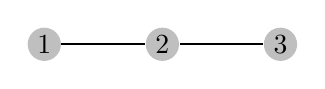
\begin{tikzpicture}[scale=1.5]
    % Draw a 7,11 network
    % First we draw the vertices
    \foreach \pos/\name in {{(1,0)/1}, {(2,0)/2}, {(3,0)/3}}
        \node[vertex] (\name) at \pos {$\name$};
    % Connect vertices with edges 
    \foreach \source/ \dest in {1/2, 2/3}
        \path[edge] (\source) -- (\dest) ;
        
\end{tikzpicture}
\end{center}

Let the $k$-threshold game with $k=3$ infinitely repeated played. Note that after nature moves, player 2 can observe the true state of nature, while player 1 or 3 are not. We can construct an APEX as followings by letting Rebel 2 reveal the state. 

\begin{itemize}
\item After nature moves, Rebel 2 (if he is) choose $\textbf{revolt}$ if he observe $\theta=(Rebel,Rebel,Rebel)$, and play \textbf{revolt} in this period. Otherwise, he choose \textbf{stay} and keep playing \textbf{stay} afterwards. 
\item After nature moves, Rebel 1 and Rebel 3 (if they are) choose \textbf{stay}.
\item If Rebel 2 choose \textbf{revolt} in the last period, then Rebel 1 (or Rebel 3) play \textbf{revolt} in this period; if Rebel 2 choose \textbf{stay} in the last period, then Rebel 1 (or Rebel 3) keep playing \textbf{stay} afterwards. 
\end{itemize}

Given the prior has full support, the above strategies constitute an equilibrium if $\delta\geq \frac{1}{2}$. In the equilibrium, Rebel 1 and Rebel 3 believe that $\{\theta:\#[Rebel](\theta)\geq 3\}$ if they observe \textbf{revolt} played by Rebel 2 and believe $\{\theta:\#[Rebel](\theta)< 3\}$ if Rebel 2 played the other action.
\end{example}

In the following section, I begin to find an APEX in more general settings.

\section{Equilibrium}
\label{sec:equilibrium}
\subsection{The case: $k=n$}

In the above special case, Example ~\ref{ex_leading_ex}, the construction of an APEX relies on some important features. First, since $k=n$ in this special case, Rebel 2 will never play \textbf{revolt} if one of his neighbour is Inert. Thus, when Rebel 2 play \textbf{revolt}, it must be the case that all Rebel 2's neighbour are Rebels. Due to this feature, Rebel 2's actions separates the states into two events, $\{\theta: \#[Rebel](\theta)\geq k\}$ and $\{\theta: \#[Rebel](\theta)< k\}$. Second, Rebel 1 or Rebel 3 can force Rebel 2 to play \textbf{revolt} to reveal the true state in the first period since only Rebel 2 knows the true state and Rebel 2's action can separate the states. Third, since $k=n$, it is easy to punish a deviation by only one Rebel's shifting to play \textbf{stay} forever, and so that the group punishment is not necessary.\footnote{For instance, if a Rebel did not play \textbf{revolt} in the second period in the state $\theta=(Rebel,Rebel,Rebel)$, his neighbour can play \textbf{stay} forever. To give incentive to let such neighbour play \textbf{stay}, we can just let the deviating player also play \textbf{stay}.} Note also that there is another APEX by letting Rebel 1 and Rebel 3 play \textbf{revolt} in the first period by using Rebel 2' punishment in shifting to play \textbf{stay} forever. I then generalize the $k=n$ case after one definition, the \textit{connectivity} of a network.

\begin{definition}
A path from $i$ to $j$ in a network $G$ is a finite sequence $k^1,...,k^q$ such that $k^1=i, k^2\in G_{k^1}\backslash k^1, k^3\in G_{k^2}\backslash k^2,...,k^q\in G_j\backslash j$. A network is connected if and only if for all $i,j$ there is a path from $i$ to $j$ or $j$ to $i$. 
\end{definition}



\begin{theorem}
\label{prop:not_crowded}
For $n$-person repeated $k$-Threshold game with parameter $k=n$ played in any network with FFCCU, then for any prior with full support there is a $\delta$ such that there is a sequential equilibrium which is approaching ex-post efficient.
\end{theorem}
\begin{proof}
The proof is constructive and is a generalization of Example. Let strategies $\tau^{*}$ as the followings. After nature moves, a Rebel play \textbf{revolt}  if there is no Inert neighbour; a Rebel play \textbf{stay} forever if there is a Inert neighbour. After first period, if a Rebel has not detected a deviation and if such Rebel observed his Rebel neighbour play \textbf{revolt} continuously in the last periods, then keep playing \textbf{revolt} in current period; otherwise, play \textbf{stay} forever. If a Rebel deviate, then himself play \textbf{stay} forever.

According to $\tau^{*}$, at period $s$, if a Rebel has not detected a deviation and if such Rebel observed his Rebel neighbour play \textbf{stay} once in the last periods, he form belief $\sum_{\theta:\#[Rebels](\theta)\geq k}\beta^{\pi,\tau^*}_{G_i}(\theta|h^{s}_{G_i})=0$ after period $s$ and therefore play \textbf{stay} after period $s$ is the best response. If a Rebel detects a deviation or himself deviate to play \textbf{stay}, play \textbf{stay} is the best response since at least one neighbour will play \textbf{stay}. \footnote{Note that we did not put additional assumptions on the off-path belief expect for the full support assumption on the prior.}

Since the network is FFCCU, there is a finite time $t^{s}_{\theta}$ such that all Rebel play \textbf{revolt} forever if $\{\theta: \#[Rebel](\theta)\geq k\}$; and there is a finite time $t^f_{\theta}$ such that all Rebel play \textbf{stay} forever if $\{\theta: \#[Rebel](\theta)< k\}$ in the equilibrium path. If a Rebel deviate, he at most get 0 after $\max\{t^{s}_{\theta},t^f_{\theta}\}$, while he get $\max\{1,0\}$ after $\max\{t^{s}_{\theta},t^f_{\theta}\}$. Due to the full support assumption, he will not deviate if $\sum_{\theta:\#[Rebels](\theta)\geq k}\beta^{\pi,\tau^*}_{G_i}(\theta|h^{s}_{G_i})>0$ at some period $s$, otherwise he has a loss in expected continuation pay-off by $\delta^{t^s_{\theta}}\frac{\sum_{\theta:\#[Rebels](\theta)\geq k}\beta^{\pi,\tau^*}_{G_i}(\theta|h^{s}_{G_i})}{1-\delta}$ after $t^s_{\theta}$. There is a $\delta_{\pi}$ such that he will not deviate.

To check if $\tau^{*}$ and $\{\beta^{\pi,\tau^*}_{G_i}(\theta|h^{s}_{G_i})\}_{i\in N}$ satisfy full consistency\footnote{Krep and Wilson (1982)}, take any $0<\eta<1$ such that Rebels play $\tau^{*}$ with probability $1-\eta$, and play others with probability $\eta$. Clearly, when $\eta \rightarrow 0$, the belief system converge to $\{\beta^{\pi,\tau^*}_{G_i}(\theta|h^{s}_{G_i})\}_{i\in N}$.
\end{proof}



\subsection{The case : $1<k<n$}

Different form the case of $k=n$, where playing \textbf{revolt} and \textbf{stay} separates the states into two events, $\{\theta: \#[Rebel](\theta)\geq k\}$ and $\{\theta: \#[Rebel](\theta)< k\}$,  this property is generally fails if  $1<k<n$. We require more assumptions on the true state and on the priors to get APEX. This is because a Rebel still have incentive to play \textbf{revolt} if there is an Inert neighbour. Moreover, Inerts will never give information to Rebels since they have only one action. Rebels' learning will be limited if some Iners block the information flow. Consider the example. 

\begin{example}\label{ex_strong_connectivity}
Let $k=2$ and let the network as the following. Assume $\theta=(Rebel_1,Inert_2,Rebel_3)$.

\begin{center}
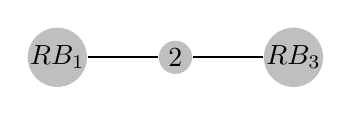
\begin{tikzpicture}[scale=1.5]
    % Draw a 7,11 network
    % First we draw the vertices
    \foreach \pos/\name in {{(1,0)/RB_1}, {(2,0)/2}, {(3,0)/RB_3}}
        \node[vertex] (\name) at \pos {$\name$};
    % Connect vertices with edges 
    \foreach \source/ \dest in {RB_1/2, 2/RB_3}
        \path[edge] (\source) -- (\dest) ;
        
\end{tikzpicture}
\end{center}

Since $k=2$, Rebel 1 has incentive to play \textbf{revolt} when $\pi(\{\theta:\theta_3=Rebel\})$ is high enough given that Rebel 3 will play revolt. Moreover, Rebel 1 never learn the true $\theta_3$ since Inert 2 block the information. We are now in the incomplete information game without communication. Clearly, the equilibrium which is APEX did not exist in this case.

\end{example}

According to Lemma ~\ref{lemma_learn}, a Rebel's belief has to learn the state of nature in APEX. Because Inerts' behaviour will not update such information, we then need to narrow down the state profiles and the prior to let APEX is possible. Define \textit{Strong connectivity} and \textit{Full support on strong connectivity} as the following.

\begin{definition}
\textbf{Strong Connectivity}: Given $G$, a state $\theta$ has strong connectivity if and only if for every pair of Rebels, there is a path consisting all Rebels to connect them.
\end{definition}  

\begin{definition}
\textbf{Full support on strong connectivity}: Given $G$, $\pi$ has full support on strong connectivity if and only if $1>\pi(\theta)>0$ whenever $\theta$ has strong connectivity.
\end{definition}  

Even if the state has strong connectivity, the coordination problem is still not trivial. Rebel may not play \textbf{stay} forever as in the case of $k=n$ if there are some Inert neighbours. With the full support assumption, they may loss the opportunity to coordinate other Rebels if they do so. Example illustrate this situation.

\begin{example}\label{ex_circle_number_5}
Let $k=5$ and let the network and the state $\theta$ as the following (the nodes other than $RB$ are Inerts).

\begin{center} 
  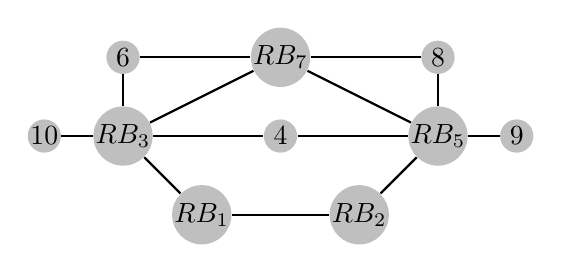
\begin{tikzpicture}[scale=1]
    % First we draw the vertices
    \foreach \pos/\name in {{(2,1)/RB_1}, {(4,1)/RB_2}, {(1,2)/RB_3}, {(5,2)/RB_5}, {(3,3)/RB_7}, {(3,2)/4}, {(1,3)/6}, {(5,3)/8}, {(6,2)/9}, {(0,2)/10}}
        \node[vertex] (\name) at \pos {$\name$};
        
%        \foreach \pos/\name in {{(3,2)/4_L}, {(1,3)/6_L}, {(5,3)/8_L}, {(6,2)/9_L}, {(0,2)/10_L}}
%   \node[selected vertex] (\name) at \pos {$\name$};
    
    % Connect vertices with edges 
    \foreach \source/ \dest in {RB_1/RB_2, RB_1/RB_3, RB_2/RB_5, RB_3/4, RB_3/6, RB_3/RB_7, 4/RB_5, RB_5/RB_7, RB_5/8, RB_5/9,6/RB_7, RB_7/8, RB_3/10}
        \path[edge] (\source) -- (\dest) ;
\end{tikzpicture}
\end{center} 

If a Rebel play stay forever, Rebels can not learn $\#[Rebels](\theta)\geq 5$. 
\end{example}

Rebels then have to find a way to communicate with each other. Their actions will be a mixture of \textbf{revolt} and \textbf{stay} in transmitting information. The construction of APEX is not trivial now because the ``dimension'' of information needed to be generated is generally larger than the cardinality of their action space. Rebels then have to use the sequence of actions to transmit information, and thus we have to track the belief updating in the time horizontal line and check if such sequences constitute an equilibrium. To see that Rebel need to generate more dimensions of information, we may compare Example ~\ref{ex_circle_number_5} and Example ~\ref{ex_circle_number_6}.
\begin{example}\label{ex_circle_number_6}
Let $k=6$ and let the network and the state $\theta_{\text{example}}$ as the following.
\begin{center} 
  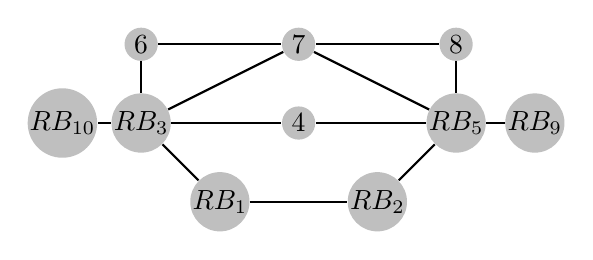
\begin{tikzpicture}[scale=1]
    % First we draw the vertices
    \foreach \pos/\name in {{(2,1)/RB_1}, {(4,1)/RB_2}, {(1,2)/RB_3}, {(5,2)/RB_5}, {(3,3)/7}, {(3,2)/4}, {(1,3)/6}, {(5,3)/8}, {(6,2)/RB_9}, {(0,2)/RB_{10}}}
        \node[vertex] (\name) at \pos {$\name$};
        
%        \foreach \pos/\name in {{(3,2)/4_L}, {(1,3)/6_L}, {(5,3)/8_L}, {(6,2)/9_L}, {(0,2)/10_L}}
%   \node[selected vertex] (\name) at \pos {$\name$};
    
    % Connect vertices with edges 
    \foreach \source/ \dest in {RB_1/RB_2, RB_1/RB_3, RB_2/RB_5, RB_3/4, RB_3/6, RB_3/7, 4/RB_5, RB_5/7, RB_5/8, RB_5/RB_9,6/7, 7/8, RB_3/RB_{10}}
        \path[edge] (\source) -- (\dest) ;
\end{tikzpicture}
\end{center} 


\end{example}

In Example, there are 6 Rebels, which is difference from Example, where there are 5 Rebels. Suppose now we have a ``talking strategies''. Rebel 3 and Rebel 5 can talk about ``how many'' Rebels in their neighbourhood to Rebel 1 and Rebel 2. Rebel 1 and Rebel 2 then talk with each other about ``how many'' Rebels they have known conditional on Rebel 3 and Rebel 5's taking. In some ways, Rebel 1 and Rebel 2 can initiate the coordination to play revolt conditional on `how many'' Rebels they have known. The question is that Rebel 1 and Rebel 2 still don't know how many Rebels out there after Rebel 3 and Rebel 5's talking. In both Example Rebel 3 and Rebel 5 will talk the same number of Rebel neighbours to Rebel 1 and Rebel 2, and Rebel 1 and Rebel 2 can not distinguish if the true number of Rebels is 5 or 6. However, if Rebel 3 and Rebel 5 can also talk about ``the locations'' of nearby Rebels, then Rebel 1 and Rebel 2 can then tell. In order to get APEX, ``talking about how many" Rebels nearby is enough, Rebels have to ``talking about the locations'' of Rebels. 

I then prepare such ``talking strategies'' to let Rebels report both the number and locations of nearby Rebels. This talking strategies is, however, not enough to get APEX. Although Lemma ~\ref{lemma_learn} shows that there is a timing such that each Rebel have known the relevant information, but it did not say that all the Rebels have known others have known the relevant information. This higher-order information hierarchy has to be commonly known before that finite time $T$ (in Definition ~\ref{Def_expost_efficient}) arrives when players play some actions repeatedly. Otherwise a tiny change in prior may let some Rebels has not arrive their $T_i$ (in Lemma), and therefore other Rebels need to form a belief about such $T_i$, and then other Rebels need to form a belief about those Rebels' belief about those $T_i$,...,and so on. Since there is no learning after $T$, this common knowledge of $T_i$ has to be formed previously\footnote{Otherwise, some Rebels may think some Rebels has not yet coordinated to some actions, and therefore those Rebels will not coordinate since some Rebels will not coordinate to some actions,...,and so on.}. 

This higher-order belief is an apparently giant object in the private imperfect monitoring setting here. By assuming the finite network, however, a preparation of \textit{coordination messages} to let Rebels talk about their $T_i$ should work. If we go back to the $k=n$ case, playing \textbf{stay} is as the role of coordination message to notify nearby Rebels the timing that coordination to \textbf{stay}, while playing \textbf{revolt} $n$ times or less (recalled that there are $n$ players) is as the coordination messages to the coordination to \textbf{revolt}. In the case of $k<n$, unfortunately, what kind of coordination message should be used in equilibrium is not obvious then. First, playing \textbf{stay} itself did not reveal $\#[Rebels](\theta)<k$ as case $k=n$ shows. Second, sending messages will incurs some expected costs (or expected benefits) and then the deviation in messages may need to be punished. It is hard to punish because the shifting to play \textbf{stay} forever is not credible or is not enough to impede the deviation now since a single Rebel's punishment may not affect the continuation pay-off and thus a group punishment may required. 

I construct the APEX with a weaker sequential consistent by assuming a off-path belief, which has a grim-trigger property. The equilibrium is constructed by three steps shown at next three subsections. In the first step, I define the \textit{information hierarchy in $G$} which gives a characterization to specify those Rebels who are forced to report their information in equilibrium, and also gives the notations in constructing my APEX. In second step, I specify Rebels' strategies as several binary $\{\textbf{revolt},\textbf{stay}\}$-sequences, and gives an automata where those binary sequences are used as inputs and outputs. Finally, I give a grim-trigger-like off-path belief in the third step and show that the sequences and automata defined in the first and second step constitute an APEX. I put the automata and the proofs in the Appendix for the convenience to read.

\subsubsection{Step 1. Information hierarchy in $G$}

The information hierarchy is defined on a network $G$ after nature choose a state but before a game is played. I will use the term ``node $i$'' instead of ``player $i$'' in this step.

The definition is by iteration. We define information hierarchy by defining $\{N^{-1}_i,N^{0}_i, N^{1}_i...\}$ and $\{I^{-1}_i,I^{0}_i, I^{1}_i...\}$ for each $i$ and each iteration in $(0,1,2,...)$, and define $\{\leq^0, \leq^1, \leq^2\}$ and $\{R^0,R^{1}, R^{2}...\}$ for each iteration in $(0,1,2,...)$. We also use the term ``blocks'' to represent the iterations.

Denote $\bar{G}_i=G_i\backslash \{i\}$ to simply notations. Given $\theta$, the information hierarchy is defined as the followings.
\begin{itemize}

\item \textbf{0-block}
Denote
\begin{eqnarray*}
N^{-1}_i &\equiv &  i \\
I^{-1}_i & \equiv & i
\end{eqnarray*}

Then define $R^0$ as 
\begin{equation}
R^0\equiv\{i:\theta_i\in[Rebels](\theta)\}
\end{equation}

\item \textbf{1-block}
Denotes
\begin{eqnarray*}
N^0_i &\equiv &  G_i \\
I^0_i & \equiv & G_i\cap R^0
\end{eqnarray*}

Define the set $\leq^0$ by defining
\begin{equation}i\in \leq^0 \Leftrightarrow \exists  j\in \bar{G}_i [I^0_i\subseteq N^0_j\cap R^0]\end{equation}  

Then define $R^1$ as 
\begin{equation}
R^{1} \equiv \{i\in R^0|i\notin \leq^0\}
\end{equation}

\item \textbf{$t+1$-block, $t\geq 1$}
Denote
\begin{eqnarray*}
N^t_i & \equiv & \bigcup_{k\in I^{t-1}_i}G_k \\
I^t_i & \equiv & \bigcup_{k\in G_i\cap R^t}I^{t-1}_k
\end{eqnarray*}


Define the set $\leq^t$ by defining
\begin{equation}i\in \leq^t \Leftrightarrow \exists j\in \bar{G}_i[I^t_i\subseteq N^t_j\cap R^0]\end{equation}

Then define $R^{t+1}$ as 
\begin{equation}
R^{t+1} \equiv  \{i\in R^t|i\notin \leq^t\}
\end{equation}


\end{itemize}

Equation shows that the $R^t$ nodes are those nodes who knows strictly more Rebels then any other their neighbours. Such nodes have the information about $I^{t-1}$ at $t$-block, which contains the updating information about who are Rebels. If any reporting incurs some expected costs, I mainly control the incentives in next two steps by just letting $R^t$ nodes to report their information, while non-$R^t$ nodes will play safe action \textbf{stay}. Moreover, if the network has no circle, it is sufficient to just let $R^t$ nodes to report information in the sense there is time $t$ and a $R^t$ node who will know the true state. 
\begin{theorem}
\label{lemma_empty}
If the network is FFCCU without circle and if the state has strong connectivity, then 
\[R^0\neq \emptyset \Rightarrow \exists t\geq 0[\exists i\in R^t[I^t_i=R^0]]\]
\end{theorem}



\subsubsection{Step 2: Equilibrium strategies in the path}


First, I assigned each player in a fixed network a distinguished prime number. Such indexation is starting from $3$. I index players $(1,2,...,n)$ as $(3,5,...,x_n)$ where $x_n$ is a prime number and the prime number assigned to $i$ will be $x_i$. Since the multiplication of distinguish prime numbers can be uniquely de-factorized as those numbers, we then use this property to let Rebels simultaneous report the number and the locations of their Rebel-neighbours by report the multiplication of those prime numbers.

There are two classes of sequences, and we call them \textit{reporting messages} and \textit{coordination messages}. I denote $\langle\rangle$ as a form of sequence. The notations for the form of those sequences are shown in Table ~\ref{Table_msg_form}. Denote $\bar{N}\subset N$ be a non-empty subset of $N$.

\begin{table}[t]
\caption{Forms of messages}
\label{Table_msg_form}
\begin{center}
\begin{tabular}{l c c}
$X_{\bar{N}}$ 								& $\equiv$ 			& $\prod_{j\in \bar{N}}x_j$  \\
\textbf{s}										& $\equiv$ 			& \textbf{stay}  \\
\textbf{r}										& $\equiv$ 			& \textbf{revolt}  \\
$\langle \textbf{stay} \rangle$ 		& $\equiv$ 			& $\langle \textbf{s},...,\textbf{s}\rangle$  \\
$\langle \textbf{revolt} \rangle$ 	& $\equiv$ 			& $\langle \textbf{r},...,\textbf{r}\rangle$  \\
$\langle  \bar{N} \rangle$ 				& $\equiv$ 			& $\langle \textbf{s},...,\textbf{s}\underbrace{\textbf{r},\textbf{s},...,\textbf{s}}_{X_{ \bar{N}}}\rangle$  \\

$\langle 1 \rangle$	 					& $\equiv$ 			& $\langle \textbf{s},...,\textbf{s}\underbrace{\textbf{r}}_{1}\rangle$  \\
$\langle \mathbf{1}_i \rangle$	 	& $\equiv$ 			& $\langle \textbf{s},...,\textbf{s}\underbrace{\textbf{r},\textbf{s},...,\textbf{s}}_{x_i}\rangle$  \\
\end{tabular}
\end{center}
\end{table}

Denote $|\langle\rangle|$ as the length of a form of sequence. The forms of sequences and the length of such forms will jointly determine the sequences I used in equilibrium. For example, if a sequence takes the form $\langle 1 \rangle$ and its length $|\langle 1 \rangle|=3$, then this sequence is $\langle \textbf{s},\textbf{s},\textbf{r}\rangle$. Thus, the length of a form is calculate from the end of such sequence.

In the equilibrium path, two kinds of periods, \textit{reporting period} and \textit{coordination period}, occur in turns in the following way,
\[\underbrace{<\text{coordination period}>}_{0-block}\underbrace{<\text{reporting period}><\text{coordination period}>}_{1-block}...\]
I.e. after nature chooses a state, all the Rebels start with $0$-block, then enter to $1$-block,...,and so on. $0$-block has only one period, coordination period. The $t$-blocks, $t\geq 1$ has two periods, reporting period and coordination period, where reporting period occurs first and then coordination period follows. The length of each period in each block is finite but endogenous.

If a sequence of actions has been played in reporting period (or coordination period), we called it a \textit{reporting messages} (or \textit{coordination messages}). In reporting period in each $t$-block ($t\geq 1$), Rebels use the sequences defined in Table to report their $I^{t-1}_i$ contingent on the histories they observed. In coordination period in each $t$-block ($t\geq 0$), Rebels check if there is one Rebel has initiate some coordination messages, which is defined in Table, and then start to coordination or continue to next reporting period in $t+1$-block. I start to give the details of these messages.



\subsubsection*{Reporting messages in reporting period}

Denote $|\langle RP^t \rangle|$ be the total number of periods in $t$-block reporting period. The outcome of pure strategies in equilibrium path take the following forms of sequences in Table ~\ref{Table_msg_reporting} with length $|\langle RP^t \rangle|$.

\begin{table}[t]
\caption{Reporting messages}
\label{Table_msg_reporting}
\begin{center}
\begin{tabular}{c c }
Reporting Messages 		&   \\
\hline
$\langle  \textbf{stay} \rangle$ 	& 	 \\
$\langle  {I^{t-1}_i} \rangle$ 		&   \\
$\langle 1 \rangle$ 		             &   \\
$\langle 2 \rangle$ 		             &   
\end{tabular}
\end{center}
\end{table}
Any deviation from the forms defined in Table ~\ref{Table_msg_reporting} will be considered as a deviation. In the equilibrium path, the beliefs a Rebel $j$ will form after observing the reporting messages by neighbour $i$ are shown in Table ~\ref{Table_blf_up_reporting}.

\begin{table}[t]
\caption{Belief updating after reporting period}
\label{Table_blf_up_reporting}
\begin{center}
\begin{tabular}{l c l}
$i$ plays 		&  			& The events $j\in \bar{G}_i$ believe with probability one  \\
\hline
$\langle  \textbf{stay} \rangle$ 	& 			    & $i\notin R^t$  \\
$\langle  {I^{t-1}_i} \rangle$ 		&  			& $i\in R^t$ and $\theta_l=Rebel$ if $l\in I^{t-1}_i$      \\
$\langle 1 \rangle$ 		             &  			& $i\in R^t$ and $i$ has known $\#[Rebels](\theta)\geq k-1$ \\
\end{tabular}
\end{center}
\end{table}

After reporting period, Rebel can tell who are $R^t$. Recall that $R^t$ Rebels are those Rebels who have strictly more information than any of their neighbours, if a Rebel $j$ have observed that none of his neighbours are in $R^t$, then he is sure that $\#[Rebels](\theta)< k$ if $\#I^{t-1}_j<k$. 

An important feature here is the usage of $\langle 1 \rangle$. It serve as a signal to indicate $i$ himself is a pivotal player and solve the free rider problem. I elaborate this issue here by providing some examples and give more details in the discussion in coordination period. As we have discussed in the Introduction, if we allow a coordination message such that every Rebels can use regardless how their reporting messages, then we have a free rider problem. Consider the Example ~\ref{ex_free_rider_tree}.

\begin{example} \label{ex_free_rider_tree}\textbf{Free Rider Problem}

Let $k=5$ and assume that there are message $\langle M_4 \rangle,\langle M_5 \rangle$ for Rebel 4, 5. To simply the analysis, let the game play starting from $1$-block, i.e. by discarding the strategies in $0$-block and staring from a reporting period. Further, assume Rebel will play \textbf{revolt} forever after observing $\langle M_4 \rangle$ or $\langle M_5 \rangle$ being played once in a period after reporting period; otherwise they will play \textbf{stay} forever. Let $G$ is as the followings.

\begin{center}
\begin{tikzpicture}[scale=1]
    % Draw a 7,11 network
    % First we draw the vertices
    \foreach \pos/\name in {{(1,2)/RB_1}, {(2,1)/RB_2}, {(2,3)/3}, {(3,2)/RB_4}, {(4,2)/RB_5}, {(5,1)/6}, {(5,3)/7}, {(6,2)/RB_8}}
        \node[vertex] (\name) at \pos {$\name$};
    
    
    % Connect vertices with edges 
    \foreach \source/ \dest in {RB_1/4, RB_2/RB_4,3/RB_4,RB_4/RB_5, RB_5/6, RB_5/7, RB_5/RB_8}
        \path[edge] (\source) -- (\dest) ;
        
\end{tikzpicture}
\end{center}

Note that Rebel 4 and Rebel 5 are $R^1$ members. Let $\langle \rangle_4$ and $\langle \rangle_5$ are the sequences of actions they may use to report the number of Rebel neighbours. These sequence will incur some expected costs. If Rebel 5 report truthfully, then Rebel 4 will not report truthfully by arranging the occurrence of \textbf{revolt}s. This is because he has a $\langle M_4 \rangle$ to initialize the coordination which all Rebels will follows by assumption. Same situation happens for Rebel 5, and then Rebel 4 and Rebel 5 will not report truthfully.

\end{example}

In the above example, two sources constitutes the free rider problem. One is that there is a coordination messages which can be used regardless the reporting messages. The other one is that Rebel 4 and Rebel 5 are pivotal in the sense that they are sure they will learn the true state given others' truthful reporting. To see the later source more clearly, consider the following Example ~\ref{ex_pivotal_1}.



\begin{example} \label{ex_pivotal_1}\textbf{Pivotal player: Case 1}
Let $k=6$ and suppose that there are message $\langle M_3 \rangle,\langle M_5 \rangle, \langle M_7 \rangle$ for Rebel 3,5,7. Let the game play starting from $1$-block as Example. Further, suppose Rebel will play \textbf{revolt} forever after observing $\langle M_3 \rangle$, $\langle M_5 \rangle$, or $\langle M_7 \rangle$ being played once in two periods\footnote{It requires two periods to let the coordination message transmit.} after reporting period; otherwise they will play \textbf{stay} forever. Let $G$ is as the followings.
\begin{center}
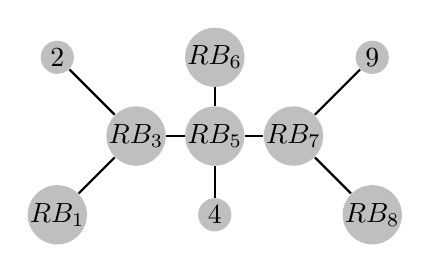
\begin{tikzpicture}[scale=1]
    % Draw a 7,11 network
    % First we draw the vertices
    \foreach \pos/\name in {{(1,1)/RB_1}, {(1,3)/2}, {(2,2)/RB_3}, {(3,1)/4}, {(3,2)/RB_5}, {(3,3)/RB_6}, {(4,2)/RB_7}, {(5,1)/RB_8}, {(5,3)/9}}
        \node[vertex] (\name) at \pos {$\name$};
    
    
    % Connect vertices with edges 
    \foreach \source/ \dest in {RB_1/RB_3, 2/RB_3,RB_3/RB_5,4/RB_5, RB_6/RB_5, RB_5/RB_7, RB_7/RB_8, RB_7/9}
        \path[edge] (\source) -- (\dest) ;
        
\end{tikzpicture}
\end{center}

Note that Rebel 3, 5, 7 are $R^1$ members. Different from Example ~\ref{ex_free_rider_tree}, although Rebel 3, 7 have coordination messages, they still have incentives to report the number of their Rebel neighbours truthfully. This is because there is a possibility that Rebel 5 misunderstood the true state if they did not report honestly, while they \textit{can not} know the true state after reporting period. Since the coordination to \textbf{revolt} has to be initiated just after reporting period, they have incentives to report truthfully.

Rebel 5, however, has no incentive to report truthfully given others' truthful reporting. This is because he is sure that he will know the true state and he can initiate the coordination given that.
\end{example}
   
Combine the issue in Example ~\ref{ex_free_rider_tree} and Example ~\ref{ex_pivotal_1} , a natural way to deal with the free rider problem is to identify who is the pivotal player in the reporting period while such pivotal player has to send the coordination messages\footnote{It is an application of Coarse Theorem}. The question is how to identify the pivotal players. If the network is FFCCU without circle, Lemma shows that the free rider problem can be identified before the game enter to $t$-block and the pivotal player can be identified either. More precisely, first define the tree rooted in $i$ node and it leaves spanning from $j\in \bar{G}_i$ as $Tr_{ij}$

\begin{definition}
$Tr_{ij}\equiv \{l\in N:\text{there is a unique path $\{l,...,j,i\}$ from $l$ to $i$ through $j$}\}$
\end{definition}
and define the set
\[C^t=\{i\in R^t:\nexists j\in R^{t-1}\cap \bar{G}_i[\exists l,l^{'}\in Tr_{ij}[l\in N^{t-1}_j\backslash I^{t-1}_i \text{ and } l^{'}\in \bar{G}_l]]\}\]
be those $R^t$ nodes so that there is no nodes connect with them more than ``two walks''. For instance, the nodes Rebel 4 and Rebel 5 in Example are $C^1$ nodes and Rebel 5 in Example is also a $C^1$ node. Then we can show the following lemmas. The proofs are in Appendix.

\begin{lemma}
\label{lemma_at_most_two_nodes}
If the network is FFCCU without circle, and  if the state has strong connectivity, then for each $t$-block
\begin{enumerate}
\item $0\leq |C^t| \leq 2$.
\item Moreover, suppose there are two nodes in $C^t$, then they are the others' neighbour.
\end{enumerate}
\end{lemma}


\begin{lemma}
\label{lemma_no_node_outside}
If the network is FFCCU without circle, and if the state has strong connectivity, then for each $t$-block
\[i\in C^t \Rightarrow \text{there is no node outside of }\bigcup_{k\in N^{t-1}_i}N_k\]
\end{lemma}

Lemma ~\ref{lemma_at_most_two_nodes} says there are at most 2 Rebels in each $t$-block and those Rebels are each others' neighbours. It is crucial because they can identify with each other by just checking the definition of $C^t$. Since they can identify with each other and since every nodes has been indexed a prime number, we just pick a node who has smaller index to be pivotal player\footnote{This property is not generally hold if a network has circle.}. Lemma ~\ref{lemma_no_node_outside} show that they can learn the true state after reporting period in $t$-block conditional on others' truthful reporting. Lemma nevertheless show only the node in $C^t$ is pivotal, and therefore there could be other nodes can learn the true state. It is troublesome because some pivotal players can not be identified before the game enter $t$-block and thus we have to identify them during the game is played by tracking the evolving information sets they face sequentially. This source to become a pivotal player is that \textit{a Rebel has already known too much}, and therefore he is sure that he will learn \textit{either $\#[Rebels](\theta)\geq k$ or $\#[Rebels](\theta)< k$} after the reporting period. Example ~\ref{ex_pivotal_2} give a more concrete example.

\begin{example} \label{ex_pivotal_2}\textbf{Pivotal player: Case 2}
Let $k=6$. Again, assume that there are coordination message $\langle M\rangle$s for Rebels. Let the game play starting from $1$-block as Example. Again, assume Rebel will play \textbf{revolt} forever after observing $\langle M \rangle$ being played once in four periods\footnote{It requires four periods to let the coordination message transmit.} after reporting period; otherwise they will play \textbf{stay} forever. Let $G$ is as the followings.

\begin{center}
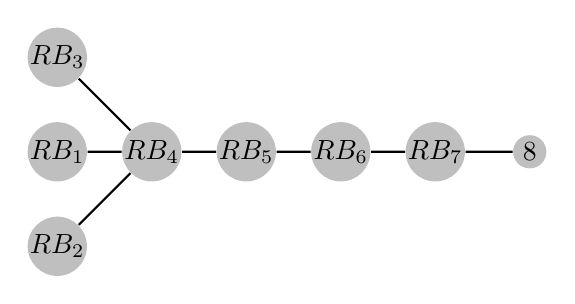
\begin{tikzpicture}[scale=1.2]
    % Draw a 7,11 network
    % First we draw the vertices
    \foreach \pos/\name in {{(2,2)/RB_1}, {(2,1)/RB_2}, {(2,3)/RB_3}, {(3,2)/RB_4}, {(4,2)/RB_5}, {(5,2)/RB_6}, {(6,2)/RB_7}, {(7,2)/8}}
        \node[vertex] (\name) at \pos {$\name$};
    
    
    % Connect vertices with edges 
    \foreach \source/ \dest in {RB_1/RB_4, RB_2/RB_4,RB_3/RB_4,RB_4/RB_5, RB_5/RB_6, RB_6/RB_7, RB_7/8}
        \path[edge] (\source) -- (\dest) ;
        
\end{tikzpicture}
\end{center}

In this case, no Rebels in $C^1$, but Rebel 4 will deviate from report $\langle I^0_4 \rangle$. Note that Rebel 4 has already known 5 Rebels in this world, so that one more Rebels is enough to initiate coordination to \textbf{revolt}. Moreover, if there is no more Rebels, the only coordination is to \textbf{stay}. If node 6 is a Rebel, Rebel 5 will report that and therefore he will know $\#[Rebels](\theta)\geq 6$. If not, due to the state has strong connectivity, he will also know $\#[Rebels](\theta)< 6$ for sure. Then he can use the message $M$ to transmit the relevant information but not report $\langle I^0_4 \rangle$.
\end{example}

After the above examples, the message $\langle 1 \rangle$ has been used to specify the pivotal players. Playing this message gives the least expected costs to distinguish themselves from non $R^t$ players. Overall speaking, the pivotal players is identified by those Rebels (1.) who have already known there are $k-1$ Rebels (sequentially) in the equilibrium path, or (2.) who are in $C^t$. The pivotal players $i$ will play $\langle 1 \rangle$ in such cases and so that the beliefs after observing it is that \textit{$i$ has known $\#[Rebels](\theta)$} in the equilibrium path, as Table ~\ref{Table_blf_up_reporting} shows.




\subsubsection*{Coordination messages in coordination period}

The ignorance of reporting messages after observed a coordination message $\langle M \rangle$ may incur the untruthfully reporting as the above examples show. The introducing of messages $\langle 1 \rangle$ is meant to tackle with that. However, one may have observed that these two messages $\langle 1 \rangle$, $\langle M \rangle$ themselves are another ``coordination message'', i.e. $\langle\langle \textbf{s}, \textbf{r} \rangle\langle M \rangle\rangle$ by truncating previous actions of $\langle 1 \rangle$ and concatenate them to $\langle M \rangle$. If the contingent behaviour after observing this new coordination message is the same as seeing the original one, the problem did not solve. In this section, I still call $\langle 1 \rangle$ as reporting messages and call those $\langle M \rangle$ as coordination messages, but I let the belief a Rebel will from contingent not only on the coordination message itself but also on reporting message.


There are three divisions in coordination period and there are several sub-blocks in each division. The form is
\[\langle\underbrace{\langle \cdot \rangle \cdot \cdot \cdot \langle \cdot \rangle}_{\text{$n$ sub-blocks}}\rangle \langle\underbrace{\langle \cdot \rangle \cdot \cdot \cdot \langle \cdot \rangle}_{\text{$t+1$ sub-blocks}} \rangle \langle\underbrace{\langle \cdot \rangle \cdot \cdot \cdot \langle \cdot \rangle}_{\text{$n$ sub-blocks}}\rangle\] 
, where $n=\# N$. Denote $CD^t_{m,n}$ be the $m$ sub-block in $n$ division, and denote $|\langle CD^t_{m,n} \rangle|$ be the total number of periods in $CD^t_{m,n}$.  The outcome of pure strategies in equilibrium path takes the following forms of sequences with length $|\langle CD^t_{m,n} \rangle|$ as Table ~\ref{Table_msg_coordination} shows.
\begin{table}[t]
\caption{Coordination messages}
\label{Table_msg_coordination}
\begin{center}

\begin{tabular}{cc }
Coordination messages		&   \\
\hline
$\langle \mathbf{1}_i \rangle$ 	& 	 \\
$\langle \textbf{stay} \rangle$	&   \\
\textbf{r}									& 	\\
\textbf{s}									& 	\\
\end{tabular}
\end{center}
\end{table}

The belief a Rebel $j$ form after observing $i$ after $CD^t_{1,1}$ in equilibrium path is as Table ~\ref{Table_blf_up_cdt11} shows. After $CD^t_{1,1}$, Rebel $j$ will tell one more event: $\#[Rebels](\theta)< k$. Clearly, if this event has been observed, the $j$ will play \textbf{stay} forever. In order to transmit this information, the strategies in $C^t_{m,1}$ where $m\geq 2$ is as Table ~\ref{Table_stg_cdt21} and Table ~\ref{Table_stg_cdtm1} shows. That is, they will play $\langle \mathbf{1}_i \rangle$ unless they observe some one play $\langle \textbf{stay} \rangle$. After $CD^t_{n,1}$, the information of $\#[Rebels](\theta)< k$ will be transmitted across all players. 
\begin{table}[t]
\caption{Belief updating after $CD^t_{1,1}$}
\label{Table_blf_up_cdt11}
\begin{center}
\begin{tabular}{c c c}
In $RP^t$ 	&  	In $CD^t_{1,1}$		&  \\
\hline
\hline
$i$ plays 		&  	$i$ plays		& The events $j\in \bar{G}_i$ believe with probability one  \\
\hline
$\langle  \textbf{stay} \rangle$ 	& 	$\langle \mathbf{1}_i \rangle$	    & $i\notin R^t$ \\
$\langle  {I^{t-1}_i} \rangle$ 		&  $\langle \textbf{stay} \rangle$		& $\#[Rebels](\theta)< k$     \\
$\langle  {I^{t-1}_i} \rangle$ 		&  $\langle \mathbf{1}_i \rangle$		& $i\in R^t$     \\
$\langle 1 \rangle$ 		             &  $\langle \textbf{stay} \rangle$		& $\#[Rebels](\theta)< k$  \\
$\langle 1 \rangle$ 		             &  $\langle \mathbf{1}_i \rangle$		&  $\#[Rebels](\theta)\geq k$ \\
$\langle 2 \rangle$ 		             &  $\langle \textbf{stay} \rangle$		&  $\#[Rebels](\theta)\geq k$ 
\end{tabular}
\end{center}
\end{table}



\begin{table}[t]
\caption{In-path strategies in $CD^t_{2,1}$}
\label{Table_stg_cdt21}
\begin{center}
\begin{tabular}{c c c}
In $RP^t$ 	 	&  	In $CD^t_{1,1}$		&  In $CD^t_{2,1}$	\\
\hline
\hline
$i$ plays 		  							&  	$i$ plays									& $j\in \bar{G}_{i}$ plays  \\
\hline
$\langle  \textbf{stay} \rangle$ 	& 	$\langle \mathbf{1}_i \rangle$	    & $\langle \mathbf{1}_i \rangle$ \\
$\langle  {I^{t-1}_i} \rangle$ 		&  $\langle \textbf{stay} \rangle$		& $\langle \textbf{stay} \rangle$     \\
$\langle  {I^{t-1}_i} \rangle$ 		&  $\langle \mathbf{1}_i \rangle$		& $\langle \mathbf{1}_i \rangle$     \\
$\langle 1 \rangle$ 		             &  $\langle \textbf{stay} \rangle$		& $\langle \textbf{stay} \rangle$  \\
$\langle 1 \rangle$ 		             &  $\langle \mathbf{1}_i \rangle$		&  $\langle \mathbf{1}_i \rangle$ \\
$\langle 2 \rangle$ 		             &  $\langle \textbf{stay} \rangle$		&  $\langle \mathbf{1}_i \rangle$ 
\end{tabular}
\end{center}
\end{table}

\begin{table}[t]
\caption{In-path strategies after $CD^t_{m,1}$, where $m\geq 2$}
\label{Table_stg_cdtm1}
\begin{center}
\begin{tabular}{c c c}
In $CD^t_{m,1}$, $m\geq 2$ 	 	&  	In $CD^t_{m+1,1}$,$m\geq 2$		& 	\\
\hline
\hline
$i$ plays 		  							&  $j\in \bar{G}_{i}$ plays  								& \\
\hline
$\langle \mathbf{1}_i \rangle$ 	& 	$\langle \mathbf{1}_i \rangle$	    &  \\
$\langle \textbf{stay} \rangle$		&  $\langle \textbf{stay} \rangle$	&  \\

\end{tabular}
\end{center}
\end{table}



Game enter to $CD^t_{1,2}$. In $CD^t_{1,2}$, Rebels start to initiate the coordination to \textbf{revolt}. The coordination message to initiate the coordination is $\langle \textbf{stay} \rangle$. As Table ~\ref{Table_blf_up_cdt12} shows, the features here is that $\langle \textbf{stay} \rangle$ is a coordination message \textit{only if} (1) $\langle  {I^{t-1}_i} \rangle$ (2) or $\langle 1 \rangle$ has been played in reporting period. Such coordination message did not occur expected costs in coordination period, but it did incur some expected costs in the reporting period. That is to say initiating the coordination to \textbf{revolt} is not free, there is a trade-off between reporting something and reporting nothing in the reporting period. This is the major force to let Rebels to report in the equilibrium path. After the initiating in $CD^t_{1,2}$, Rebels start to transmit the information of $\#[Rebels](\theta)\geq k$ in $CD^t_{m,2}$ $m\geq 2$ as Table ~\ref{Table_stg_cdt12} and Table ~\ref{Table_stg_cdtm2} shows. That is, they will play $\langle \textbf{stay} \rangle$ unless they observe some one play $\langle \mathbf{1}_i \rangle$. After $CD^t_{{t+1},1}$, the information of $\#[Rebels](\theta)\geq k$ will be transmitted across at least $k$ Rebels. We need $t+1$ sub-blocks in this stage because such $k$ Rebels are within a neighbourhood around that Rebel who initiate coordination at most $t+1$ sub-blocks.
\begin{table}[t]
\caption{Belief updating after $CD^t_{1,2}$}
\label{Table_blf_up_cdt12}
\begin{center}
\begin{tabular}{l c c c}
In $RP^t$ 	 	&  	In $CD^t_{1,1}$		&  In $CD^t_{1,2}$	  &\\
\hline
\hline
$i$ plays 		                             &  	$i$ plays		&				$i$ plays			& The events $j$ believe with probability one  \\
\hline
$\langle  \textbf{stay} \rangle$ 	& 	$\langle \mathbf{1}_i \rangle$	&  $\langle \textbf{stay} \rangle$ &  $i\notin R^t$ \\
$\langle  {I^{t-1}_i} \rangle$ 		&  $\langle \textbf{stay} \rangle$	&	$\langle \textbf{stay} \rangle$ &  $\#[Rebels](\theta)< k$   \\
$\langle  {I^{t-1}_i} \rangle$ 		&  $\langle \mathbf{1}_i \rangle$	&	$\langle \textbf{stay} \rangle$ &  $\#[Rebels](\theta)\geq k$    \\
$\langle  {I^{t-1}_i} \rangle$ 		&  $\langle \mathbf{1}_i \rangle$	&	$\langle \mathbf{1}_i \rangle$ &  $i\in R^t$  \\
$\langle 1 \rangle$ 		             &  $\langle \textbf{stay} \rangle$	&	$\langle \textbf{stay} \rangle$ &  $\#[Rebels](\theta)< k$\\
$\langle 1 \rangle$ 		             &  $\langle \mathbf{1}_i \rangle$	&	$\langle \textbf{stay} \rangle$ & $\#[Rebels](\theta)\geq k$\\
$\langle 2 \rangle$ 		             &  $\langle \textbf{stay} \rangle$	&	$\langle \textbf{stay} \rangle$ &  $\#[Rebels](\theta)\geq k$
\end{tabular}
\end{center}
\end{table}




\begin{table}[t]
\caption{In-path strategies in $CD^t_{2,2}$}
\label{Table_stg_cdt12}
\begin{center}
\begin{tabular}{l c c c}
In $RP^t$ 	 	&  	In $CD^t_{1,1}$		&  In $CD^t_{1,2}$	  & In $CD^t_{2,2}$ \\
\hline
\hline
$i$ plays 		                             &  	$i$ plays		&				$i$ plays			& $j\in \bar{G}_i$ plays  \\
\hline
$\langle  \textbf{stay} \rangle$ 	& 	$\langle \mathbf{1}_i \rangle$	&  $\langle \textbf{stay} \rangle$ &  $\langle \textbf{stay} \rangle$ \\
$\langle  {I^{t-1}_i} \rangle$ 		&  $\langle \textbf{stay} \rangle$	&	$\langle \textbf{stay} \rangle$ &  $\langle \textbf{stay} \rangle$   \\
$\langle  {I^{t-1}_i} \rangle$ 		&  $\langle \mathbf{1}_i \rangle$	&	$\langle \textbf{stay} \rangle$ &  $\langle \mathbf{1}_i \rangle$    \\
$\langle  {I^{t-1}_i} \rangle$ 		&  $\langle \mathbf{1}_i \rangle$	&	$\langle \mathbf{1}_i \rangle$ &  $\langle \textbf{stay} \rangle$  \\
$\langle 1 \rangle$ 		             &  $\langle \textbf{stay} \rangle$	&	$\langle \textbf{stay} \rangle$ &  $\langle \textbf{stay} \rangle$\\
$\langle 1 \rangle$ 		             &  $\langle \mathbf{1}_i \rangle$	&	$\langle \textbf{stay} \rangle$ & $\langle \mathbf{1}_i \rangle$\\
$\langle 2 \rangle$ 		             &  $\langle \textbf{stay} \rangle$	&	$\langle \textbf{stay} \rangle$ &  $\langle \mathbf{1}_i \rangle$
\end{tabular}
\end{center}
\end{table}

\begin{table}[t]
\caption{In-path strategies after $CD^t_{m,2}$, where $m\geq 2$}
\label{Table_stg_cdtm2}
\begin{center}
\begin{tabular}{c c c}
In $CD^t_{m,2}$, $m\geq 2$ 	 	&  	In $CD^t_{m+1,2}$,$m\geq 2$		& 	\\
\hline
\hline
$i$ plays 		  							&  $j\in \bar{G}_{i}$ plays  								& \\
\hline
$\langle \mathbf{1}_i \rangle$ 	& 	$\langle \mathbf{1}_i \rangle$	    &  \\
$\langle \textbf{stay} \rangle$		&  $\langle \textbf{stay} \rangle$	&  \\

\end{tabular}
\end{center}
\end{table}






Game finally enter to $CD^t_{1,3}$. In this period, those $k$ Rebels who have known the information of $\#[Rebels](\theta)\geq k$ will start to play \textbf{revolt} forever. This is the first period to get positive expected pay-off by playing \textbf{revolt} if the coordination can be succeeded to \textbf{revolt}. After $CD^t_{m,3}$, $m\geq 2$, other Rebels start to transmit this information of coordination to \textbf{revolt} to all of the Rebels as Table ~\ref{Table_stg_cdm3} shows.

\begin{table}[t]
\caption{In-path strategies in $CD^t_{1,3}$}
\label{Table_stg_cd13}
\begin{center}
\begin{tabular}{c c c}
In $CD^t_{m,2}$, $1\leq m\leq t+1$ 	 	&  	In $CD^t_{1,3}$		& 	\\
\hline
\hline
$i$ has played 		  							&  $j\in \bar{G}_{i}$ plays  								& \\
\hline
$\langle \mathbf{1}_i \rangle$ 	& 	\textbf{r}	    &  \\
Otherwise		&  \textbf{s}	&  \\

\end{tabular}
\caption{In-path strategies after $CD^t_{m,3}$, where $m\geq 2$}
\label{Table_stg_cdm3}
\end{center}
\end{table}

\begin{table}[t]
\begin{center}
\begin{tabular}{c c c}
In $CD^t_{m,3}$, $m\geq 2$ 	 	&  	In $CD^t_{m+1,3}$, $m\geq 2$		& 	\\
\hline
\hline
$i$ plays 		  							&  $j\in \bar{G}_{i}$ plays  								& \\
\hline
\textbf{r} 	& 	\textbf{r}	    &  \\
\textbf{s}		&  \textbf{s}	&  \\

\end{tabular}
\end{center}
\end{table}



\subsubsection{Step 3: Off-path Belief and Incentives In-the-path}

Whenever a deviation is detected by Rebel $i$ at period $s$, he form the belief $\beta^{\pi,\tau}_{G_i}(\bar{\theta}|h^{s}_{G_i})=1$ for all $s^{'}\geq s$, where $\bar{\theta}=\times_{j\in G_i}\{\theta_j\}\times_{j\notin G_i}\{Inert\}$. Thus, if $\# I^0_i<k$, he will play \textbf{stay} forever and this is credible after $1$-block. This off-path belief then serve as a grim trigger to impede Rebels' deviation. Then I check if this grim trigger can sustain my APEX. The details are given in the Appendix.

Though the grim trigger strategy highly reduce players' incentives to deviate, a downside of using grim trigger strategy to sustain a APEX in this framework is due to the pay-off function is not continuous at Rebel's revolting. Recall that a APEX require \text{all} the players to play ex-post efficient outcome, not just $k$ players. If the judgement for a deviation is too strict, such equilibrium may not be sustained by grim trigger since a deviation may be only detected by some Rebels, while there may be at least $k$ Rebels can not detect it, and therefore there are $k$ Rebels play \textbf{revolt} forever, while the others play \textbf{stay} for ever. This phenomenon gives another reason in explaining why the message $\langle 1 \rangle$ needed to be introduced. Consider the Example ~\ref{ex_deviation} (, a modification of Example ~\ref{ex_pivotal_1}).

\begin{example}\label{ex_deviation}
Let $k=5$ and suppose that there are message $\langle M_3 \rangle,\langle M_5 \rangle, \langle M_7 \rangle$ for Rebel 3,5,7. Let the game play starting from $1$-block as Example. Suppose Rebel will play \textbf{revolt} forever after observing $\langle M_3 \rangle$, $\langle M_5 \rangle$, or $\langle M_7 \rangle$ \textit{if no deviation be detected}; otherwise they will play \textbf{stay} forever. Moreover, assume that Rebels can only use the pure strategies in which the outcome satisfies the form of $\langle I^0_i \rangle$ in reporting period; \textit{otherwise, it  will be consider as deviation}. 

Let the players be indexed by prime numbers $x_i$ in network $G$ in Figure and suppose the $\theta$ is as Figure.
\begin{center}
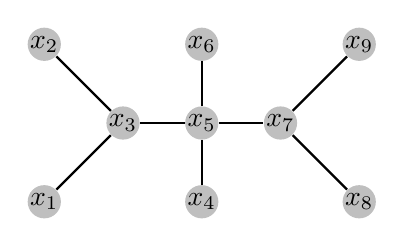
\begin{tikzpicture}[scale=1]
    % Draw a 7,11 network
    % First we draw the vertices
    \foreach \pos/\name in {{(1,1)/x_1}, {(1,3)/x_2}, {(2,2)/x_3}, {(3,1)/x_4}, {(3,2)/x_5}, {(3,3)/x_6}, {(4,2)/x_7}, {(5,1)/x_8}, {(5,3)/x_9}}
        \node[vertex] (\name) at \pos {$\name$};
    
    
    % Connect vertices with edges 
    \foreach \source/ \dest in {x_1/x_3, x_2/x_3,x_3/x_5,x_4/x_5, x_6/x_5, x_5/x_7, x_7/x_8, x_7/x_9}
        \path[edge] (\source) -- (\dest) ;
        
\end{tikzpicture}
\end{center}



\begin{center}
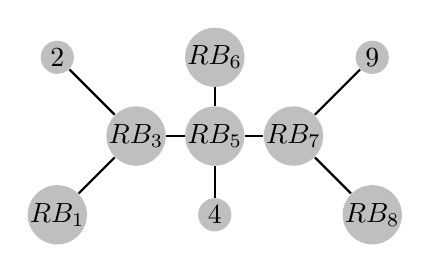
\begin{tikzpicture}[scale=1]
    % Draw a 7,11 network
    % First we draw the vertices
    \foreach \pos/\name in {{(1,1)/RB_1}, {(1,3)/2}, {(2,2)/RB_3}, {(3,1)/4}, {(3,2)/RB_5}, {(3,3)/RB_6}, {(4,2)/RB_7}, {(5,1)/RB_8}, {(5,3)/9}}
        \node[vertex] (\name) at \pos {$\name$};
    
    
    % Connect vertices with edges 
    \foreach \source/ \dest in {RB_1/RB_3, 2/RB_3,RB_3/RB_5,4/RB_5, RB_6/RB_5, RB_5/RB_7, RB_7/RB_8, RB_7/9}
        \path[edge] (\source) -- (\dest) ;
        
\end{tikzpicture}
\end{center}

Assume $X_{I^0_3}>X_{I^0_5}$ and $X_{I^0_7}>X_{I^0_5}$. Rebel 5 will get the information from Rebel 3,7 before his reporting of $I^0_5$. Rebel 5 will not report $I^0_5$, although there is a punishment, since he can deviate to report $\bar{I}^0_5=x_3\times x_5\times x_7<I^0_5$ by not letting Rebel 3, 7 detect, while the coordination can be succeeded. Rebel 6 can detect such deviation since the de-factorization of $X_{\bar{I}^0_5}$ did not include his own index $x_6$. However, Rebel 6 will then keep play \textbf{stay} forever although the coordination has been succeeded.

\end{example}

Due to the pay-off function is not continuous, a Rebel is more willing to report his information if he still don't know there are at least $k$ Rebels, while he is less willing after he has known that. More Rebels to join a coordination did not change his pay-off.  The criteria in judging deviation should not be too strict as Example shows. Otherwise, in the lack of other ``paths'' to be considered as the equilibrium path, some Rebels will be excluded from coordination with this grim-trigger-like strategies. The messages, $\langle 1 \rangle$, are then introduced to give more paths in the equilibrium path along with this grim trigger strategies. In previous subsections, I have listed the belief updating in equilibrium path by showing the the belief after observing various messages, the proof in Appendix is then to show an APEX, which can be sustained by this off-path belief.

\subsection{Result}
\label{sec:result}

The goal of this paper is to show that there is always an APEX in a network given that the network is FFCCU without circle.
\begin{theorem}
\label{thm_main_result}
For $n$-person repeated $k$-Threshold game with parameter $1\leq k \leq n$ played in any FFCCU network without cycle,
if the state $\theta$ has strong connectivity and $\pi(\{\theta: \theta\text{ has strong connectivity}\})=1$ with full support, then there is a $\delta$ such that there is a (weak) sequential equilibrium which is approaching ex-post efficient.
\end{theorem}

The proof is in Appendix. The argument at first is to use off-path belief to impede players from deviating from the form of sequences and then get a clear learning process in the path. Then I argue that any deviation without detection (and therefore no punishment from other player) before a Rebel knows $\#[Rebels](\theta)\geq k$ or $\#[Rebels](\theta)< k$ will create noise in impeding the learning process, which will lower down expected continuation pay-off, and therefore such deviation will punish themselves. Finally, by the equilibrium construction in coordination period, most profitable deviation in the coordination period can be detected, and therefore Rebels can be forced by off-path belief to transmit coordination message  to all Rebels after some Rebels knows $\#[Rebels](\theta)\geq k$ or $\#[Rebels](\theta)< k$. To see that an undetectable deviation can impede the learning process, consider the case when a Rebel want to pretend himself as a pivotal player. According to Table and Table, the continuation playing contingent on observing $\langle 1 \rangle$ is either playing \textbf{stay} forever or \textbf{revolt} forever after current block. This repeated playing will then block the information updating. By full support assumption and by the similar argument in the proof in Theorem, when $\delta$ is high enough, he is better off by staying in the equilibrium path where the true state of nature can be learnt.

This equilibrium still can be founded in some variations of the games. I consider the case when pay-off is not hidden and the case when Rebels have different levels of efforts when they contribute to a collective action. The two subsections below discusses these variations.

\subsubsection{Variation: Pay-off as signals}
The pay-off has been assumed to be hidden in the previous analysis, but it can be relaxed without change the result in Theorem. One may consider that there is a noise to impede Rebels to observe their static pay-off. For example, what they fight for is to gather international attention, however, the autocrat block and manipulate the international news. Or, for instance, the outcome of revolution may depend not only on their joint efforts but also on another effect, says the weather, and therefore the joint efforts did not guarantee the successfulness but it give higher expected pay-off. 

One may consider there are two public signals, $y_1,y_2$, generated by Rebels' actions.
\begin{eqnarray*}
p_{1s} &=& \mathrm {Pr}(y_1|\#\textbf{revolt}\geq k) \\
p_{1f} &=& \mathrm {Pr}(y_1|\#\textbf{revolt}< k) \\
p_{2s} &=& \mathrm {Pr}(y_2|\#\textbf{revolt}\geq k) \\
p_{2f} &=& \mathrm {Pr}(y_2|\#\textbf{revolt}< k) 
\end{eqnarray*}
with
\begin{equation}
p_{1s}u_{y_1,\textbf{revolt}}+p_{2s}u_{y_2,\textbf{revolt}}>0>p_{1f}u_{y_1,\textbf{revolt}}+p_{2f}u_{y_2,\textbf{revolt}}
\end{equation}
\begin{equation}
1>p_{1s}>0,1>p_{2s}>0,p_{1f}=1-p_{1s},p_{2f}=1-p_{2s}
\end{equation}

Equation (6) is a generalization of previous setting, where $0$ still represent the pay-off by playing a safe action, \textbf{stay}. Equation (7) is a full support assumption on the signals of $y=\{y_1,y_2\}$.

With the full support assumption as Equation (7), we can construct the same equilibrium strategies as previous analysis by ignore the noisy signal $y$. By directly checking the equilibrium strategy, the major force to impede players from making undetectable deviation is that his deviation will let himself more uncertain about the true state, and therefore he should stay in the path to learn the true state. 

However, if Equation (7) fails and so that the pay-off can be perfectly observed, says $p_{1s}=p_{2f}=1$, the equilibrium constructed above will be no more an equilibrium. A Rebel will just send $\langle 1 \rangle$ and wait to see if the pay-off is getting to $1$ by other players' playing in the equilibrium path (recall Table and Table). It is a profitable deviation since Rebels then keep playing revolt if they have observed the pay-off of $1$. In this case, however, it is easy to construct another APEX by letting all Rebels play \textbf{revolt} in the first period, and then keep playing \textbf{revolt} or \textbf{stay} contingent on the signals $y$.

\subsubsection{Variation: Rebels with different levels of efforts}

We can also consider a model in which players have different levels of efforts in contributing a collective action. Let the enlarged space of states of nature as $\hat{\Theta}=\Theta \times \Xi$, where $\Xi=\{1,2,...,k\}^n$. A $\hat{\theta}=(\theta,e)$, where $\theta\in \Theta$ and $e\in \Xi$, is interpreted as a state of nature in which a player $i$ could be either a Rebel or Inert with levels of effort $e_i$, where $e_i\in \{1,...,k\}$. A Rebel playing \textbf{revolt} is interpreted as a contribution to a collective action, while such collective action require $k$ amount of efforts. If such collective action succeed, a Rebel $i$ will get an amount of $b_i>0$ as his reward. Thus, we have a variation in pay-off structure as
\begin{enumerate}
\item $u_{Rebel}(a_i,a_{-i})=b_i$ if $a_i=\textbf{revolt}$ and $\sum_{j:a_j=\textbf{revolt}}e_j\geq k$
\item $u_{Rebel}(a_i,a_{-i})=-e_i$ if $a_i=\textbf{revolt}$ and $\sum_{j:a_j=\textbf{revolt}}e_j< k$
\item $u_{Rebel}(a_i,a_{-i})=0$ if $a_i=\textbf{stay}$
\item $u_{Inert}(a_i,a_{-i})=1$ if $a_i=\textbf{inert}$
\end{enumerate}

The things matter here is that the states of nature should be discrete, and therefore we can use prime indexing to construct the equilibrium as previous result shows.

\section{Discussion}
\label{sec:discuss}

The implicit technique in my equilibrium construction is that the pivotal Rebels can be identified before the game is played each reporting period in each block. When the network has circle, the selection of pivotal Rebels need more elaboration. 
\begin{example}\label{ex_free_rider_circle}
Let $k=6$. Suppose the network and $\theta$ is as the following. 




\begin{center}
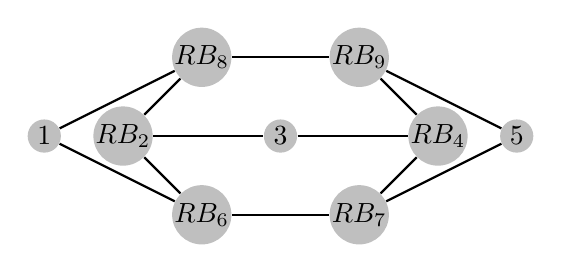
\begin{tikzpicture}[scale=1]
    % Draw a 7,11 network
    % First we draw the vertices
    \foreach \pos/\name in {{(1,3)/1}, {(2,3)/RB_2}, {(4,3)/3}, {(6,3)/RB_4}, {(7,3)/5}, {(3,2)/RB_6}, {(5,2)/RB_7}, {(3,4)/RB_8}, {(5,4)/RB_9}}
        \node[vertex] (\name) at \pos {$\name$};
    
    
    % Connect vertices with edges 
    \foreach \source/ \dest in { 1/RB_6, 1/RB_8, RB_2/3, RB_2/RB_8, 3/RB_4, RB_2/RB_6, RB_6/RB_7, RB_8/RB_9, RB_9/RB_4, RB_7/RB_4, RB_9/5, RB_7/5}
        \path[edge] (\source) -- (\dest) ;
        
\end{tikzpicture}
\end{center}

Assume that one round of reporting is done. Rebel 2 has known $\{RB_2,RB_6,RB_8,RB_9,RB_7\}$, Rebel 4 has known $\{RB_4,RB_7,RB_9,RB_8,RB_6\}$, and so on. One more round of reporting will let Rebels 3,6,7,4,9,8 knows the true state $\theta$, and therefore Rebels 3,6,7,4,9,8 are all pivotal Rebels conditional on others truthful reporting. We may have a rule as Example by picking up a pivotal Rebel dependent on its prime number index, say we pick Rebel 4. However, this selection of pivotal players is ex-post. The true state $\theta^{'}$ could be as 

\begin{center}
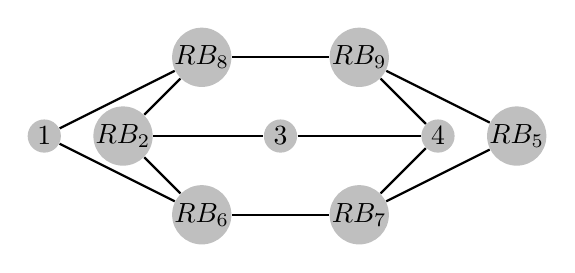
\begin{tikzpicture}[scale=1]
    % Draw a 7,11 network
    % First we draw the vertices
    \foreach \pos/\name in {{(1,3)/1}, {(2,3)/RB_2}, {(4,3)/3}, {(6,3)/4}, {(7,3)/RB_5}, {(3,2)/RB_6}, {(5,2)/RB_7}, {(3,4)/RB_8}, {(5,4)/RB_9}}
        \node[vertex] (\name) at \pos {$\name$};
    
    
    % Connect vertices with edges 
    \foreach \source/ \dest in { 1/RB_6, 1/RB_8, RB_2/3, RB_2/RB_8, 3/4, RB_2/RB_6, RB_6/RB_7, RB_8/RB_9, RB_9/4, RB_7/4, RB_9/RB_5, RB_7/RB_5}
        \path[edge] (\source) -- (\dest) ;
        
\end{tikzpicture}
\end{center}

Now node 4 is an Inert and so that he is not a pivotal Rebel. Some other rules are needed to selection a Rebel (say, Rebel 5 in this case) during the game is played. 

\end{example}

As Example ~\ref{ex_free_rider_circle} shows, a free rider problem may occur if the selection of pivotal Rebels is not done before the game is played. When the network has circle, this problem seems more harsh and the selection rule may not be done before the game is played. Though it is possible to prove that if such selection  fails, says an Inert has been selected (as the Inert 4 in the above example), then the other Rebels can take over it (as the Rebel 5 in the above example), the proof is still infeasible in this paper. 

Another free rider problem may occur when the underlying network has circles is that a Rebel's information can be covered by another Rebel, and therefore it reduce the incentives to report such information if reporting information incurs expected costs. However, this problem can be dealt with by our construction of reporting messages and by the assumption that the network is commonly known. 

\begin{example}
Let $k=6$. Rebel 3 and Rebel 4 have the same information $I^1_3=I^1_4$. Since reporting is costly, if there is no punishment, Rebel 3 (or Rebel 4) may shirk and deviate from truthfully reporting if Rebel 4 (or Rebel 3) can reports truthfully. However, this kind of deviation can be detected by Rebel 5 (or Rebel 2) since $I^1_3$ should be equal to $I^1_4$. 

\begin{center}
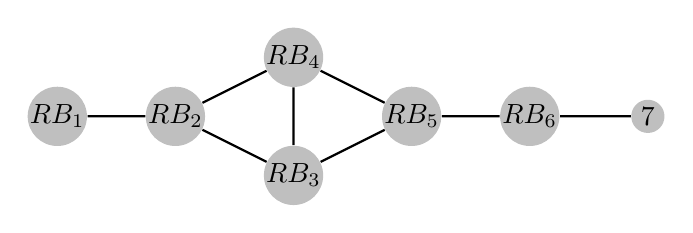
\begin{tikzpicture}[scale=1.5]
    % Draw a 7,11 network
    % First we draw the vertices
    \foreach \pos/\name in {{(1,2)/RB_1}, {(2,2)/RB_2}, {(3,1.5)/RB_3}, {(3,2.5)/RB_4}, {(4,2)/RB_5}, {(5,2)/RB_6}, {(6,2)/7}}
        \node[vertex] (\name) at \pos {$\name$};
    
    
    % Connect vertices with edges 
    \foreach \source/ \dest in {RB_1/RB_2, RB_2/RB_3,RB_2/RB_4,RB_3/RB_5, RB_4/RB_5, RB_5/RB_6, 7/RB_6, RB_4/RB_3}
        \path[edge] (\source) -- (\dest) ;
        
\end{tikzpicture}
\end{center}


Indeed, this monitoring technique will be less invalid if the network is not commonly known. If Rebels has asymmetric information about network structure, says Rebel 5 (or Rebel 2,3) did not certain if there is a link between Rebel 4 and Rebel 2, then Rebel 4 can just pretend that he didn't know Rebel 2\footnote{However, with asymmetric information about network structure, the Example is less than a free rider problem. Dependent on given asymmetric information, Rebel 3 and Rebel 4 then have different incentives in untruthful reporting, which may be a dominant strategy for Rebel 4 but not necessary be a dominant strategy for Rebel 3.}. The analysis in incomplete information about network structure is beyond the scope of this paper. Recent paper such as [].

\end{example}

















\section{Conclusion}
\label{sec:con}

Which individuals can be coordinators to guide the whole society to an efficient outcome depends on the location of such individual. From example, in a not-crowded network, the non-spike players are coordinators; in a centipedes, the spine players play such roles. Since network is commonly known, individuals can know where are those coordinators and trace the information flow along with the network. Especially, in a not-crowded network in Section ~\ref{sec:results}, everyone is a coordinator. Combine the above results, if one want to relax the common knowledge assumption, says the game being played in a random network, the analysis have to consider the uncertainty about individuals' allocation and their role to transmit the information. 

To change a network also means to change the initial information about the true state in this model. This feature may link the existing Graph Theory literature to analyze how incomplete information affects in repeated game (such as \cite{sorin1996}).  We may also think a inhabitant can strategically form the link to others, so that they can gather information aggressively. That is to combine the result in network formation literature \cite{JAsurvey2003} and the literature in incomplete information repeated game, then to understand the dynamic information aggregation.

\bibliographystyle{abbrvnat}	% (uses file "plain.bst")
\bibliography{jmp_ref}		% expects file "myrefs.bib"


\appendix
\section{Appendix}

\textbf{proof for Theorem ~\ref{lemma_empty}}
\begin{proof}
This proof follow three useful claims, Claim ~\ref{lemma_I_subset_N}, Claim ~\ref{lemma1} and Claim ~\ref{lemma_connected}. To simplify notation, denote $\bar{G}_i=G_i\backslash \{i\}$. First note that $I^t_i$ can be expressed as 
\begin{equation}
\label{eq_info_nb}
I^{t}_i = \bigcup_{k_0\in N_i\cap R^{t}}\bigcup_{k_1\in N_{k_0}\cap R^{t-1}}...\bigcup_{k_{t-1}\in N_{k_{t-2}}\cap R^{1}}N_{k_{t-1}}\cap R^0
\end{equation}
, while $H^t_i$ can be expressed as
\begin{equation}
\label{eq_nb}
N^t_i = \bigcup_{k_0\in N_i\cap R^{t-1}}\bigcup_{k_1\in N_{k_0}\cap R^{t-2}}...\bigcup_{k_{t-2}\in N_{k_{t-3}}\cap R^{1}}N_{k_{t-2}}
\end{equation}

\begin{claim}
\label{lemma_I_subset_N}
$I^t_i\subset N^t_i$, $I^t_i=\bigcup_{k\in I^{t-1}_i}N_k\cap R^0$, and $N^t_i=\bigcup_{k\in N^{t-1}_i}N_k$ for all $t\geq 0$.
\end{claim}
\begin{proof}
$I^t_i\subset N^t_i$ is by definition. $I^t_i=\bigcup_{k\in I^{t-1}_i}N_k\cap R^0$ and $N^t_i=\bigcup_{k\in N^{t-1}_i}N_k$ is by comparing Equation ~\ref{eq_info_nb} and Equation ~\ref{eq_nb}.
\end{proof}

\begin{claim}
\label{lemma1}
If the network is FFCCU without circle, then for each $t\geq 1$ block, we have $i\in R^t\Leftrightarrow i\in R^{t-1} \text{ and } \exists k_1,k_2\in R^{t-1}\cap \bar{G}_i$, where $k_1\neq k_2$.
\end{claim}
\begin{proof}
The proof is by induction. We first show that the statement is true for $t=1$. 

\textbf{Base}: $i\in R^1\Leftrightarrow [i\in R^0] \wedge [\exists k_1,k_2\in (R^0\cap \bar{G}_i)]$. 

$\Rightarrow$: Since $i\in R^1$, then $i\in R^0$ and then $I^0_i\nsubseteq N^0_j$ for all $j\in \bar{G}_i$ by definition. Since $I^0_i=R^0\cap G_i$, then $\forall j\in \bar{G}_i [\exists k\in (R^0\cap \bar{G}_i) [k\notin N^0_j]]$. Since the $j\in \bar{G}_i$ is arbitrary,  we then have a pair of $k_1, k_2 \in (R^0\cap \bar{G}_i)$ such that $k_1\notin N^0_{k_2}$ and $k_2\notin N^0_{k_1}$.

$\Leftarrow$: Pick $k\in \{k_1,k_2\}\subseteq (R^0\cap \bar{G}_i)$, and pick an arbitrary $j\in \bar{G}_i\backslash \{k\}$. Note that $k\notin N^0_j$, otherwise there is a circle from $i$ to $i$. Hence $[k\in (R^0\cap \bar{G}_i)] \wedge [k\notin N^0_j]$ and therefore $[k\in I^0_i] \wedge [k\notin N^0_j]$. Then we have $I^0_i\nsubseteq N^0_j$ for arbitrary $j\in \bar{G}_i$, and thus $i\in R^1$.

\textbf{Induction hypothesis}: the statement is true for $\{1,2,..,t\}$ where $t\geq 1$. 


If the hypothesis is true, then $i\in R^{t+1}\Leftrightarrow [i\in R^{t}] \wedge [\exists k_1,k_2\in (R^{t}\cap \bar{G}_i)]$


$\Rightarrow$: since $i\in R^{t+1}$, then $i\in R^t$ and $I^t_i\nsubseteq N^t_j$ for all $j\in \bar{G}_i$ by definition. Recall that $I^t_i$ can be expressed as $I^{t}_i = \bigcup_{k_0\in N_i\cap R^{t}}\bigcup_{k_1\in N_{k_0}\cap R^{t-1}}...\bigcup_{k_{t-1}\in N_{k_{t-2}}\cap R^{1}}N_{k_{t-1}}\cap R^0$ and $H^t_i$ can be expressed as $N^t_i = \bigcup_{k_0\in N_i\cap R^{t-1}}\bigcup_{k_1\in N_{k_0}\cap R^{t-2}}...\bigcup_{k_{t-2}\in N_{k_{t-3}}\cap R^{1}}N_{k_{t-2}}$, then for every $l\in I^{t-1}_i$, we can find a path connecting $i$ to $l$ by the induction hypothesis. If $j\in \bar{G}_i$, then we can find a path connecting $j$ to $l$ by connecting $j$ to $i$, and then connecting $i$ to $l$. Thus, if $l\in I^{t-1}_i$ then $l\in N^t_J$, and hence $I^{t-1}_i\subseteq N^t_{j}$ for all $j\in \bar{G}_i$. Recall that $I^t_i = \bigcup_{k\in N_i\cap R^t}I^{t-1}_k$ and $i\in R^{t+1}$, then we must have $\forall j\in \bar{G}_i [\exists k\in (R^t\cap \bar{G}_i)[ I^{t-1}_k\nsubseteq N^t_j]]$, since $I^{t-1}_i\subseteq N^t_{j}$. Note that such $j\in \bar{G}_i$ is arbitrary,  we then have a pair of $k_1, k_2 \in (R^{t}\cap \bar{G}_i)$ such that $k_1\notin N^t_{k_2}$ and $k_2\notin N^t_{k_1}$.
\bigskip

$\Leftarrow$:
By the induction hypothesis, we have a chain $k_{1_0},...,k_{1_t},i,k_{2_t},...,k_{2_0}$ with $k_{1_0}\in R^0$,..., $k_{1_t}\in R^t$, $i\in R^t$, $k_{2_t}\in R^t$,...,$k_{1_0}\in R^0$, where $k_{1_t},k_{2_t}\in (R^{t}\cap \bar{G}_i)$, $k_{1_0}\in I^{t-1}_{k_{1_t}}$ and $k_{2_0}\in I^{t-1}_{k_{2_t}}$. Note that $k_{1_0}\notin N^t_j$ whenever $j\in \bar{G}_i$, otherwise there is a circle from $i$ to $i$ since $\{i,k_{2_t},...,k_{2_0}\}\in N^t_j$, and hence $[k_{1_0}\in I^{t-1}_{k_{1_t}}] \wedge [k_{1_0}\notin N^t_j]$ for all $j\in \bar{G}_i$. Therefore we have $[I^{t-1}_{k_{1_t}}\in I^t_i] \wedge [I^{t-1}_{k_{1_t}}\notin N^t_j]$ for all $j\in \bar{G}_i$ since $k_{1_t},k_{2_t}\in (R^{t}\cap \bar{G}_i)$ and $[k_{1_0}\in I^{t-1}_{k_{1_t}}] \wedge [k_{1_0}\notin N^t_j]$ for all $j\in \bar{G}_i$. Then we have $I^t_i=\bigcup_{k\in N_i\cap R^{t}}I^{t-1}_k\nsubseteq N^t_j$ for arbitrary $j\in \bar{G}_i$, and thus $i\in R^{t+1}$.



We can then conclude that the statement is true by induction.




\end{proof}



\begin{claim}
\label{lemma_connected}
If the network FFCCU without circle and if the state has strong connectivity, then if there is a pair of $R^{t}$ nodes then there exists a $R^{t}$-path connecting them.
\end{claim}
\begin{proof}
The proof is by induction and by Claim ~\ref{lemma1}. Since the state has strong connectivity, we have a $R^0$-path connecting each pair of $R^0$ nodes. Since all pairs of $R^0$ nodes are connected by a $R^0$-path, then for all pairs of $R^1$ nodes must be in some of such paths by Claim ~\ref{lemma1}, and then connected by a $R^0$-path. But then all the $R^0$-nodes in such path are all $R^1$ nodes by Claim ~\ref{lemma1} again and by $R^t\subseteq R^{t-1}$ for $t\geq 1$ by definition. Thus, for all pairs of $R^1$ nodes has a $R^1$-path connecting them. The similar argument holds for $t> 1$, we then get the result.

\end{proof}
I begin to prove this Theorem ~\ref{lemma_empty}. I first claim that if $R^t\neq \emptyset$ and if $R^{t+1}= \emptyset$, then $R^0\subset I^t_i$ whenever $i\in R^t$. Then I claim that if $R^t\neq \emptyset$ then $\# R^{t+1}<\# R^t$. Finally, I iterate $R^t$ with $t\geq 0$ to get the conclusion.

If $R^t\neq \emptyset$ but $R^{t+1}= \emptyset$, I claim that $R^0\subset I^{t}_i$ for all $i\in R^t$. The proof is by contradiction. If $R^0\not\subset I^{t}_i$, there is a $j\in R^0$ but $j\notin I^t_i$. Since $I^t_i=\bigcup_{k_0\in N_i\cap R^{t}}\bigcup_{k_1\in N_{k_0}\cap R^{t-1}}...\bigcup_{k_{t-1}\in N_{k_{t-2}}\cap R^{1}}N_{k_{t-1}}\cap R^0$, then there is no such a path $\{i,k_0,k_1,...,k_{t-1},j\}$, where $k_0\in G_i\cap R^{t},k_1\in G_{k_0}\cap R^{t-1},...,k_{t-1}\in N_{k_{t-2}}\cap R^{1}$. Since $R^{t+1}=\emptyset$ and therefore $R^{t^{'}}=\emptyset$ if $t^{'}\geq t+1$, and hence there is no such a path containing a node in $R^{t^{'}}=\emptyset$, where $t^{'}\geq t+1$ connecting $i$ to $j$. But $i\in R^t$ and $i,j\in R^0$, if there is no such a path, then it violate either Claim ~\ref{lemma_connected} or Claim ~\ref{lemma1}. Contradiction.

Next I claim that if $R^t\neq \emptyset$ then $\# R^{t+1}<\# R^t$. The proof is the followings. Given a node $i$ in $R^t$, let $j\in R^t$ (could be $i$ itself) be the node connected with $i$ with the maximum shortest $R^t$ path. This $j$ can be found since $R^t\neq \emptyset$ and the network is finite. Then there is no $R^t$ node in $j$'s neighbourhood other than the nodes in this path. Since the network is without circle, there is at most one $R^t$ node in $j$'s neighbourhood. But then $j\notin R^{t+1}$ since it violate Claim ~\ref{lemma1}.

Starting from $R^0\neq \emptyset$ and iterating $R^t$ with $t\geq 0$, if $R^t\neq \emptyset$ but $R^{t+1}= \emptyset$, then there is some $i$ with $R^0\subset I^t_i$ as the above paragraph shows; if $R^t\neq \emptyset$ and $R^{t+1}\neq \emptyset$, then we starting from $R^{t+1}$ and iterating $R^{t+1}$ with $t\geq t+1$. Since $\#R^{t+1}<\#R^t$ as the above paragraph shows, there is a time $t^{*}$ with $R^{t^{*}}=\emptyset$, then we get the conclusion.


\end{proof}




\textbf{proof for Lemma ~\ref{lemma_at_most_two_nodes}}

\begin{proof}
Denote $(i,j)$-path as the set of paths from $i$ to $j$. The proof is by contradiction. Suppose there are three or more $R^t$-nodes in $C^t$, then pick any three nodes of them, and denote them as $i_1,i_2,i_3$. Let's say $i_2$ is in a $(i_1,i_3)$-path by strong connectivity, and therefore $i_2\in Tr_{i_1i_2}$ and $i_3\in Tr_{i_2i_3}$. First we show that $i_1\in G_{i_2}$ (or $i_3\in G_{i_2}$). Suppose $i_1\notin N_{i_2}$, since $i_1,i_2\in R^t$, then the $(i_1,i_2)$-path is a $R^t$-path by Claim ~\ref{lemma1}. Let this $(i_1i_2)$-path be $\{i_1,j_1,...,j_n,i_2\}$. Since $i_1,j_1,...,j_n,i_2\in R^t$, we then have $I^{t-1}_{i_1}\nsubseteq N^{t-1}_{j_1},...,I^{t-1}_{j_n}\nsubseteq N^{t-1}_{i_2}$ and $I^{t-1}_{j_1}\nsubseteq N^{t-1}_{i_1},...,I^{t-1}_{i_2}\nsubseteq N^{t-1}_{j_n}$. Since $I^{t-1}_{i_1}\subseteq N^{t-1}_{i_1},...,I^{t-1}_{i_2}\subseteq N^{t-1}_{i_2}$ by Lemma ~\ref{lemma_I_subset_N}, we further have $\exists k_1\in R^0[k_1\in N^{t-1}_{j_1}\backslash I^{t-1}_{i_1}]$,...,$\exists k_n\in R^0[k_n\in N^{t-1}_{j_n}\backslash I^{t-1}_{i_2}]$. Since the state has strong connectivity, there is a $R^0$ path connecting $k_1,...,k_n$ by Claim ~\ref{lemma_connected}. But then we have already found $k_1,k_2$ such that $k_1\in N^{t-1}_{j_1}\backslash I^{t-1}_{i_1}$ and $k_2\in \bar{G}_{k_1}$. It is a contradiction that $i_1\in C$.

Now, $i_1,i_2,i_3$ will form a $R^t$-path as $\{i_1,i_2,i_3\}$. With the same argument as the above, we then have $\exists k_1\in R^0[k_1\in N^{t-1}_{i_2}\backslash I^{t-1}_{i_1}]$ and $\exists k_2\in R^0[k_2\in N^{t-1}_{i_3}\backslash I^{t-1}_{i_2}]$, and thus $i_1$ is not in $C$.
\end{proof}


\textbf{proof for Lemma ~\ref{lemma_no_node_outside}}
\begin{proof}
The proof is by contradiction. Since $i\in R^t$, there is a $j\in (R^{t-1}\cap \bar{G}_i)$ by Lemma ~\ref{lemma1}. Note that $N^{t-1}_j\subseteq \bigcup_{k\in N^{t-1}_i}N_k$ since $N^{t-1}_j =\bigcup_{k\in I^{t-2}_j}N_k$, and $I^{t-2}_j\subseteq I^{t-1}_i\subseteq N^{t-1}_i$. If there is another node outside $\bigcup_{k\in N^{t-1}_i}N_k$ in $Tr_{ij}$, then there must be another node such that there is a path connected to some nodes in $N^{t-1}_j$ since the network is connected. It is a contradiction that $i\in C$.

\end{proof}

\subsection{Equilibrium}

\subsubsection{Out-off-path belief}

If Rebel $i$ detects a deviation at $m$ period, he form the belief as
\begin{equation}
\beta_{i}(\{\theta:\theta\in \times_{j\in G_i}\{\theta_j\}\times\{Inert\}^{n-\#G_i}\}|h^{m^{'}}_{G_i})=1 \text{ , } m^{'}\geq m
\end{equation}



\subsubsection{Equilibrium Path: Notations}


\begin{itemize}

\item $\langle \rangle_r$ be the set of finite sequence of actions in which the action \textbf{r} occurs once and only once.
\item $PF(\langle \rangle,m)$ be the $m$-periods prefix of $\langle \rangle$.
\item $(i,j)$-path be the set of paths from $i$ to $j$.

\end{itemize}

\subsubsection{Equilibrium Path: reporting period}

\paragraph{reporting period: notations}
\begin{itemize}
\item $m$ be a period in reporting period.
\item $|\langle RP^t \rangle|$ be the total periods in reporting period in $t$-block
\item $O^{m,t}_i$ be the set of $i$'s neighbours $j$s who has played a sequence $M$ such that $M=PF(\langle I^{t-1}_j \rangle,m)$ and $M \in \langle \rangle_r$ at $m$ period in the reporting period of $t$-block 
\item $I^{m,t}_i\equiv (\bigcup_{k\in O^{m,t}_i} I^{t-1}_k)\cup I^{t-1}_i$ be the updated relevant information gathered by $i$ at period $m$ in the reporting period of $t$-block. Note that $I^{0,t}_i=I^{t-1}_i$ and $I^{|\langle RP^t|,t \rangle}_i=I^{t}_i$.
\item $N^{m,t}_i\equiv (\bigcup_{k\in O^{m,t}_i} N^{t-1}_k)\cup N^{t-1}_i$
be the updated neighbourhood which contains $I^{m,t}_i$

\item Let 
\[Ex_{I^{m,t}_i}\equiv \{l\notin N^{m,t}_i|\exists l^{'}\in I^{m,t}_i\text{ such that there exists a $(l,l^{'})$-path}\}\]
be all the possible Rebel nodes outside of $N^{m,t}_i$ given $I^{m,t}_i$
\item Let
\[Tr_{I^{m,t}_ij}\equiv Tr_{ij}\cap (Ex_{I^{m,t}_i}\cup I^{m,t}_i)\]
be all the possible Rebel nodes in the $Tr_{ij}$ given $I^{m,t}_i$. 
\end{itemize}
\paragraph{reporting period: automata}
\subparagraph{$i\notin R^{t}$}




\begin{itemize}
\item \textbf{WHILE LOOP}
\begin{itemize}
\item At $m\geq 0$, if $\#Ex_{I^{m,t}_i}\cup I^{m,t}_i< k$, report $\langle \textbf{stay} \rangle$ and then play \textbf{stay} forever.
\item Otherwise, \textbf{runs POST-CHECK }
\end{itemize}
\end{itemize}

\subparagraph{$i\in R^{t}$}

\begin{itemize}

\item \textbf{WHILE LOOP}
\begin{itemize}
\item At $m\geq 0$, if $\# Ex_{I^{m,t}_i}\cup I^{m,t}_i< k$, report $\langle \textbf{stay} \rangle$ and then play \textbf{stay} forever.
\item Otherwise, \textbf{runs MAIN }
\end{itemize}


\item \textbf{MAIN}

At $m\geq 0$, 

\begin{enumerate}
\item At $m=0$ and if $\# I^{t-1}_i=\# I^{0,t}_i= k-1$, then 
\textbf{runs POST-CHECK }


\item At $m=0$ and if $i\in R^t$ and
\[\nexists j\in R^{t-1}\bar{G}_i \text{ such that }\exists l_1,l_2\in Tr_{ij}[[l_1\in N^{t-1}_j\backslash I^{t-1}_i] \wedge [l_2\in \bar{G}_{l_1}]]]\]
, then runs \textbf{CHECK.$0$}. Otherwise, recall \textbf{MAIN}
\item At $0\leq m \leq |RP^t|-|\langle I^{t-1}_i \rangle|$, play
\[\textbf{stay}\]
\item At $m = |RP^t|-|\langle I^{t-1}_i \rangle|+1$, then
\begin{enumerate}
\item if $O^{m,t}_i= \emptyset$ 
, then report
\[\langle I^{t-1}_i \rangle\]
\item if $O^{m,t}_i\neq \emptyset$, then \textbf{runs CHECK.k}

\end{enumerate}

\end{enumerate}





\item \textbf{CHECK.$0$}

At $m=0$, if $i\in C$, i.e. if $i\in R^t$ and
\[\nexists j\in R^{t-1}\cap \bar{G}_i \text{ such that }[\exists l_1,l_2\in Tr_{ij}[[l_1\in N^{t-1}_j\setminus I^{t-1}_i] \wedge [l_2\in \bar{G}_{l_1}]]]\]
, then
\begin{enumerate}
\item If $\#C=1$
, then 
\textbf{runs POST-CHECK }

\item If $\#C=2$, then denote $i_1,i_2\in C$ such that $I^{t-2}_{i_1}<I^{t-2}_{i_2}$, and then
\begin{itemize}
\item if $i=i_1$, then 
\textbf{runs POST-CHECK }
\item if $i=i_2$, then report
\[\langle I^{t-1}_i \rangle\]

\end{itemize}
\end{enumerate}




\item \textbf{CHECK.$m$}

 At $m>0$, if $O^{m,t}_i\neq \emptyset$, then there are two cases, 
\begin{enumerate}
\item Case 1: If $i\in R^t$ and 
\[\exists j\in  O^m_i \text{ such that }\exists l_1,l_2\in Tr_{I^{m,t}_ij}[[l_1\in I^{t-1}_j\backslash I^{t-1}_i] \wedge [l_2\in \bar{G}_{l_1}]]]\]
, then report 
\[\langle I^{t-1}_i \rangle\]
\item Case 2: If $i\in R^t$ and 
\[\not\exists j\in  O^m_i \text{ such that }\exists l_1,l_2\in Tr_{I^{m,t}_ij}[[l_1\in I^{t-1}_j\backslash I^{t-1}_i] \wedge [l_2\in \bar{G}_{l_1}]]]\]

\begin{enumerate}
\item Case 2.1: If $i\in R^t$ and 
\[\not\exists j\in R^{t-1}\cap (G_i\backslash  O^{m,t}_i) \text{ such that }[\exists l_1,l_2\in Tr_{I^{m,t}_ij}[[l_1\in N^{t-1}_j\backslash I^{t-1}_i] \wedge [l_2\in \bar{G}_{l_2}]]]\]
\[\textbf{Note: this case is the case when $i\in C$, thus recall Check.0}\]

\item Case 2.2: If 
\[\exists j\in R^{t-1}\cap (G_i\backslash  O^{m,t}_i) \text{ such that }[\exists l_1,l_2\in Tr_{I^{m,t}_ij}[[l_1\in N^{t-1}_j\backslash I^{t-1}_i] \wedge [l_2\in \bar{G}_{l_2}]]]\]

\begin{itemize}
\item if $\# I^{m,t}_i= k-1$
, then 
\textbf{runs POST-CHECK }

\item if $\# I^{m,t}_i< k-1$
, then report 
\[\langle I^{t-1}_i \rangle\]
\end{itemize}





\end{enumerate}

\end{enumerate}





\item \textbf{CHECK.k}

At $m\geq 1$, 
\begin{enumerate}


\item $O^{m,t}_i\neq \emptyset$, and
 \[\# I^{m,t}_i\geq k\]
, then 
\textbf{runs POST-CHECK }

\item $O^{m,t}_i\neq \emptyset$, and 
\[ \#I^{m,t}_i< k\]
, then \textbf{runs CHECK.$m$}
\end{enumerate}


\item \textbf{POST-CHECK}

\begin{enumerate}


\item At $m=|RP^t|$, then
\begin{enumerate}
\item If $i\in R^t$ and if $|I^{m,t}_i|\geq k-1$, then play
\textbf{revolt}

\item if $i\notin R^t$, then play
\textbf{stay}


\end{enumerate}
\end{enumerate}


\end{itemize}



\subsubsection{Equilibrium path: coordination period}
\paragraph{coordination period: notations}
\begin{itemize}
\item $m$ be a sub-block in coordination period.
\item Let 
\[Ex_{I^{t}_i}\equiv \{l\notin I^{t}_i|\exists l^{'}\in I^{t}_i\setminus I^{t-1}\text{ such that there exists a $(l,l^{'})$-path}\}\]
be all the possible Rebel nodes outside of $N^{t}_i$ given $I^{t}_i$.

\item Let
\[Tr_{I^{t}_ij}\equiv Tr_{ij}\cap (Ex_{I^{t}_i}\cup I^{t}_i)\]
be the set of possible Rebel nodes in the $Tr_{ij}$ given $I^{t}_i$. 

\end{itemize}




\paragraph{coordination period: automata}


\begin{itemize}





\item \textbf{1st Division} 


In 1st division, for $t\geq 0$ block and for $1\leq m \leq n$ sub-block,
\begin{itemize}

\item If $i$ has played $\langle 1 \rangle$, then play
\[\langle \mathbf{1}_i \rangle\]

\item If $\# Ex_{I^{t}_i}\cup I^{t}_i<k$, then \[\langle\textbf{play $l$ forever}\rangle\]

\item If $\# Ex_{I^{t}_i}\cup I^{t}_i\geq k$, and there are some $j\in \bar{G}_i$ have played $\langle \textbf{stay} \rangle $, then play
\[\left\{
\begin{array}{l r l}      
    \langle \mathbf{1}_i \rangle \text{ and then runs \textbf{COORDINATION}} 	& \text{if } &\# I^{0}_i\geq k \\
    \langle\textbf{play $l$ forever}\rangle														&\text{if } 		& \text{otherwise}
\end{array}\right.
\]
\item If $\# Ex_{I^{t}_i}\cup I^{t}_i \geq k$, and there is no $j\in \bar{G}_i$ has played $\langle \textbf{stay} \rangle $, then play
\[\langle \mathbf{1}_i \rangle\]

\end{itemize}




\item \textbf{2nd Division} 

If there is no $j\in G_i$ such that $j$ has played $\langle \textbf{stay} \rangle$ in the \textbf{1st Division} , then run the following automata. Otherwise, $\langle\textbf{play $l$ forever}\rangle		$ 

\begin{itemize}
\item $i\notin R^t $
\begin{itemize}
\item In the $1$-sub-block: play
\[\langle \textbf{stay} \rangle \]


\item In the $2\leq m\leq t+1$ sub-blocks: 

\begin{enumerate}

\item If $i\in R^{t^{'}}$ for some $t^{'}\geq 0$ and if there is a $j\in R^{t^{'}+1}\cap \bar{G}_i$ has played 
\begin{enumerate}
\item $\langle \textbf{stay} \rangle $ in $m=1$ sub-block
\item or $\langle \mathbf{1}_j \rangle$ in $m\geq 2$ sub-blocks
\end{enumerate}
, then play 
\[\langle \mathbf{1}_i \rangle\] in $m+1$ sub-block.

\item Otherwise, play
\[\langle \textbf{stay} \rangle\] in current sub-block
\end{enumerate}

\end{itemize}

\item $i\in R^t$

\begin{itemize}
\item In the $1$-sub-block:
\begin{enumerate}
\item If $i$ has played $\langle 1 \rangle$, then play
\[\langle \textbf{stay} \rangle \]

\item If $i$ has not played $\langle 1 \rangle$ and if there is a $j\in \bar{G}_i$ has played $\langle 1 \rangle$, then play
\[\langle \textbf{stay} \rangle \]

\item If $i$ has not played $\langle 1 \rangle$ and if there is no $j\in \bar{G}_i$ has played $\langle 1 \rangle$, then
\begin{itemize}
\item If $\# I^{|RP^t|,t}_i\geq k$, then play
\[\langle \textbf{stay} \rangle \]
\item If $\# I^{|RP^t|,t}_i< k$, then play
\[\langle \mathbf{1}_i  \rangle \]
\end{itemize}

\end{enumerate}

\item In the $m\geq 2$-sub-block: 

\begin{enumerate}

\item If $i\in R^{t^{'}}$ for some $t^{'}\geq 0$ and if there is a $j\in R^{t^{'}}\cap \bar{G}_i$ has played 
\begin{enumerate}
\item $\langle \textbf{stay} \rangle$ in $m=1$ sub-block, or
\item $\langle \mathbf{1}_j \rangle$ in $m\geq 2$ sub-blocks
\end{enumerate}
, then play 
\[\langle \mathbf{1}_i \rangle\] in $m+1$ sub-block.
\item Otherwise, play
\[\langle \textbf{stay} \rangle\] in current sub-block.
\end{enumerate}

\end{itemize}

\end{itemize}



\item \textbf{3rd Division} 

\begin{enumerate}
\item \textbf{INITIATING} 

If $i$ has observed $j\in N_i\setminus i$ has played,
\begin{enumerate}
\item $\langle \textbf{stay} \rangle$ in $1$-sub-block in pre-coordination period or
\item $\langle \mathbf{1}_j \rangle$ in $m\geq 2$ sub-blocks in pre-coordination period or
\item $\langle h \rangle$ in the \textbf{3rd Division} 
\end{enumerate}
, then play
\[\langle \textbf{play $h$ forever} \rangle\]
\item \textbf{NOT INITIATING} 

Otherwise, play 
\textbf{stay} 
in current period.
\end{enumerate}
\end{itemize}





\subsubsection{proof for Theorem ~\ref{thm_main_result}}

To simplify the notations, if $P(\theta)$ is a property of $\theta$, then abuse the notations by letting $\beta^{\pi,\tau^*}_{G_i}(P(\theta)|h^{m}_{G_i})\equiv \sum_{\theta:P(\theta)}\beta^{\pi,\tau^*}_{G_i}(\theta|h^{m}_{G_i})$. We say ``$i$ knows $P(\theta)$'' by means of $\beta^{\pi,\tau^*}_{G_i}(P(\theta)|h^{m}_{G_i})=1$.

\paragraph{Equilibrium path: proof}
\begin{claim}
\label{claim_either_success_or_fail}
In the equilibrium path and for $\#Ex_{I^{m,t}_i}\cup I^{m,t}_i\geq k$, where $m$ is a period in reporting period. If $i$ report $\langle 1 \rangle$, then either coordinate to \textbf{revolt} after $t$-block or $\# R^0<k$.
\end{claim}
\begin{proof}
By directly checking the equilibrium path, we have
\begin{enumerate}
\item if $\# I^{|RP^t|,t}_i\geq s$, then the coordination can be initiated by such $i$.
\item if $\# I^{|RP^t|,t}_i= k-1$, and if there is one more node who reported $\langle 1 \rangle$, then the coordination can be initiated by $i$.
\item if $\# I^{|RP^t|,t}_i= k-1$, and if there are no nodes who reported in current period, then $\# I^{|RP^t|,t}_i=\# I^{t}_i= k-1$. We now check the conditions guiding $i$ to \textbf{POST-CHECK}.
\begin{itemize}
\item If $i$ is coming from the conditions in \textbf{MAIN}, it means that there is no further $H$-node outside $I^{t-1}_i$, and thus outside $\bigcup_{k\in I^{t-1}_i}G_k$.
\item If $i$ is coming from the conditions in \textbf{CHECK.0}, it means that there is no further $H$-node outside $\bigcup_{k\in I^{t-1}_i}G_k\cap R^0$, and thus outside $\bigcup_{k\in I^{t-1}_i}G_k$. 
\item If $i$ is coming from the conditions in \textbf{CHECK.m}, it means that there is no further $H$-node outside $\bigcup_{k\in I^{t-1}_i}G_k\cap R^0$, and thus outside $\bigcup_{k\in I^{t-1}_i}G_k$. 
\end{itemize}
Then $\# I^{t}_i< k$, but $I^t_i=\bigcup_{k\in I^{t-1}_i}N_k\cap R^0$, and hence $\# R^0<k$.

\end{enumerate}


\end{proof}



\begin{lemma}
If the state has strong connectivity, then for all $n$-person repeated $k$-Threshold game with parameter $1\leq k\leq n$ played in any finite connected undirected network without circle, the equilibrium path is approaching efficient.
\end{lemma}

\begin{proof}
We want to show that when $\theta$ satisfying $\#[Rebels](\theta)\geq k$, all the Rebels play \textbf{revolt} eventually; when $\theta$ satisfying $\#[Rebels](\theta)< k$, all the Rebels play \textbf{stay} eventually.
\begin{enumerate}
\item If all the Rebels only play $\langle I^{t-1} \rangle$ or $\langle \textbf{stay} \rangle$ in reporting period for all $t\geq 1$ block, then by the equilibrium path, those nodes played $\langle I^{t-1} \rangle$ are $R^t$-node, and those nodes played $\langle \textbf{stay} \rangle$ are not-$R^t$ nodes. 

If there are some Rebels play $\langle \textbf{stay} \rangle$ in the first division in $t$-block, then all the Rebels play \textbf{stay} eventually; If $R^t$ Rebels play $\langle \textbf{stay} \rangle$ in the first sub-block in second division in $t$-block, then all the Rebels will play \textbf{stay} after third division in this block. Otherwise, all the Rebels go to the next reporting period.

By Theorem ~\ref{lemma_empty}, there is a $t^{*}$ such that there is a $R^{t^{*}}$ node knows $\theta$, and therefore he knows if $\theta$ satisfying $\#[Rebels](\theta)\geq k$ or $\#[Rebels](\theta)< k$. In equilibrium path, such node play $\langle \textbf{stay} \rangle$ either in the first sub-block in first division or in the first sub-block in second division in coordination period.Thus the equilibrium path is approaching efficient.

\item If there are some Rebels play $\langle 1 \rangle$ in reporting period for a $t\geq 1$ block, then by Claim ~\ref{claim_either_success_or_fail}, such nodes will knows if $\theta$ satisfying $\#[Rebels](\theta)\geq k$ or $\#[Rebels](\theta)< k$ after reporting period in this $t$-block. Then $\langle \textbf{stay} \rangle$ is either played in the first sub-block in first division or played in the first sub-block in second division in coordination period. Thus the equilibrium path is approaching efficient.

 
\end{enumerate}

\end{proof}



\paragraph{No deviation: proof in reporting period}


\begin{claim} 
\label{claim_detection_reporting_period}
For $\#Ex_{I^{m,t}_i}\cup I^{m,t}_i\geq s$. Denote $D$ be the set of Rebels who detect $i$'s deviation. If $\# I^{m,t}_i<k$. If $D\neq \emptyset$, then there is a $\delta$ such that $i$ will not deviate.
\end{claim}
\begin{proof}

Denote $D$ be the set of neighbours who detect $i$'s deviation. Let the events be
\begin{eqnarray*}
E_1 	&= &\{\theta: \#[Rebels](\theta)< k\}\\
E_2 	&= &\{\theta: k\leq \#[Rebels](\theta)<k+\# D\}\\
E_3 	&= &\{\theta: \#[Rebels](\theta)\geq k+\# D\}
\end{eqnarray*}

In equilibrium path, there are periods $t^{s}$ ($t^{f}$) such that if $\theta$ satisfying $\#[\text{Rebels}](\theta)\geq k$ ( $\#[\text{Rebels}](\theta)< k$) then Rebels play \textbf{revolt} (\textbf{stay}) forever. If $i$ follows the equilibrium path, the expected static pay-off after $\max\{t^s,t^f\}$\footnote{There is $t^{s}$ or $t^{f}$ for each $\theta$. The maximum is among those possible $\theta$.} is
 \[\beta_{i}(E_2|h^{m}_{N_i})+\beta_{i}(E_3|h^{m}_{N_i})\]

If $i$ deviate, the expected static pay-off after $\max\{t^s,t^f\}$ is
 \[\beta_{i}(E_3|h^{m}_{N_i})\]
 
Therefore there is a loss in expected static pay-off of
\[\beta_{i}(E_2|h^{m}_{N_i})\]

Thus, there is a loss in expected continuation pay-off contingent on $E_2$ by
\[\delta^{\max\{t^s,t^f\}}\frac{\beta_{i}(E_2|h^{m}_{N_i})}{1-\delta}\]

\end{proof}



\begin{claim} 
\label{claim_deviation_higher_reporting}
For $\# Ex_{I^{m,t}_i}\cup I^{m,t}_i \geq k$. If $\# I^{m,t}_i<k$, there is a $\delta$ such that $i$ will not deviate by reporting $\bar{I}^{t-1}_i\neq I^{t-1}_i$ if such deviation is not detected by $i$'s neighbour.
\end{claim}

\begin{proof}
Assume $\bar{I}^{t-1}_i\neq I^{t-1}_i$. Since a detection of deviation has not occur, it must be the case that there is a non-empty set $F=\{j\in \bar{I}^{t-1}_i:\theta_j=Inerts\}$\footnote{Otherwise, there is a detection of deviation. Recall the definition in information hierarchy: $I^{-1}_i\subset I^{0}_i\subset...\subset I^{t-1}_i$ for all $i\in R^0$}. 


Let the set 
\[E_1=\{\bar{\theta}: \bar{\theta}_j=Rebel \text{ if } j\in F \text { and }\bar{\theta}_j=\theta_j \text{ if } j\notin F\}\]
be the set of pseudo events by changing $\theta_j$ where $j\in F$. And let
\[E_2=\{\theta: \theta_j=Inert \text{ if }j\in F \text { and }\bar{\theta}_j=\theta_j \text{ if } j\notin F\}\]
be the set of true event.

Then consider the event
\begin{eqnarray*}
E 	&= &\{\bar{\theta}\in E_1: \#[Rebels](\bar{\theta})\geq k\}\\
 	&= &\{\theta\in E_2: \#[Rebels](\theta)\geq k-\#F\}
\end{eqnarray*}

Partition $E$ as sub events
\begin{eqnarray*}
E_3 	&= &\{\theta\in E_2: \#[Rebels](\theta)\geq k\}\\
E_4 	&= &\{\theta\in E_2: k>\#[Rebels](\theta)\geq k-\#F\}
\end{eqnarray*}

By Lemma ~\ref{lemma_empty} and following the strategies in equilibrium path (since $i$ have not been detected), there is a block $\bar{t}^{s}$ with respect to $\bar{\theta}$ such that if $\bar{\theta}\in E$ then there some $R^{\bar{t}^s}$ Rebel $j$s, says $J$, will initiate the coordination, and then Rebels play \textbf{revolt} forever after $\bar{t}^s$-block. Note that such $j$ is with $\# {I}^{\bar{t}^{s}}_i \geq k$ by Claim.

We have several cases:
\begin{enumerate}
\item Case 1: If $i\in J$, his own initiation will only depends on $\# I^{\bar{t}^s}_i$ by Claim, which is the same as he has reported $\langle {I}^{t-1}_i\rangle$. It is strictly better by not deviating since playing $\langle\bar{I}^{t-1}_i\rangle$ is more costly than $\langle\bar{I}^{t-1}_i\rangle$ ($X_{\bar{I}^{t-1}_i}>X_{I^{t-1}_i}$).
\item Case 2: If there is another $j$ who $\bar{I}^{t-1}_i\not\subset I^{\bar{t}^{s}}_j$\footnote{Recall that }, then such $j$'s initiation of coordination dependent of his own information about $\theta$, $\subset I^{\bar{t}^{s}}_j$, by Claim and $i$'s deviation did not change $j$'s information. It is strictly better by not deviating since playing $\langle\bar{I}^{t-1}_i\rangle$ is more costly than $\langle\bar{I}^{t-1}_i\rangle$.
\item Case 3: If there is another $j$ who $\bar{I}^{t-1}_i\subset {I}^{\bar{t}^{s}}_j$ such that $\# I^{\bar{t}^s}_i\geq k$. If $i$ did not follow $j$'s initiation of coordination, then there is a detection of deviation by checking the equilibrium path. Such detection will let $i$'s continuation expected pay-off down to zero, and therefore $i$ should follow this initiation as Claim shows. If $i$ follows, and $\#I^{\bar{t}^s}_i\geq s$, we are in the Case 1. If $i$ follows, but $\#I^{\bar{t}^s}_i< s$, then $i$'s expected static pay-off after $\bar{t}^{s}$ is at most
\[
{\max\{\beta_{i}(E_3|h^{m}_{N_i})\times 1+\beta_{i}(E_4|h^{m}_{N_i})\times (-1), 0\}}
\]

However, if $i$ follow the equilibrium path, there is are $t^s$, $t^f$ such that the expected static pay-off after $\max\{t^s,t^f\}$ is
\[\max\{\beta_{i}(E_3|h^{m^{'}}_{N_i}),0\}\]

Thus, there is a loss in expected continuation pay-off contingent on $E$ by
\[\delta^{\max\{t^s,t^f\}}\frac{\min\{\beta_{i}(E_3|h^{m}_{G_i}),\beta_{i}(E_4|h^{m}_{G_i})\}}{1-\delta}\]
\end{enumerate}


\end{proof}



\begin{claim} 
\label{claim_can_not_pretend_almost_success}
For $\#Ex_{I^{m,t}_i}\cup I^{m,t}_i\geq s$. If $\#I^{m,t}_i\leq s-1$, and if $i\notin C$ or $i$ did not satisfy the condition to play $\langle 1 \rangle$, $i$ will not play $\langle 1 \rangle$.
\end{claim}


\begin{proof}


Let
\[E^{'}=\{\theta:\#I^{RP^t,t}_i\leq k-1\}\]

The event is not empty by checking the timing where $i$ deviated. We have two case:
\begin{enumerate}
\item If $i$ has a neighbour $j\in C$, then $j\not\in O^{RP^t,t}_i$, and then suppose all other neighbour are not in $R^t$.
\item If \[\exists j\in R^{t-1}\cap \bar{G}_i \text{ such that } \exists k_1,k_2\in Tr_{ij}[[k_1\in N^{t-1}_j\backslash I^{t-1}_i] \wedge [k_2\in \bar{G}_{k_2}]]\], then just let $E=\{\theta: N^t_i\cap R^0\leq k-1\}=\{\theta: I^t_i\leq k-1\}=E^{'}$\footnote{note that $I^t_i$=$I^{RP^t,t}_i$}.
\end{enumerate}

Next, let 
\begin{eqnarray*}
E_1&=&\{\theta: \#[Reble](\theta)<k\}\cap E^{'}\\
E_2&=&\{\theta: \#[Reble](\theta)\geq k\}\cap E^{'}\\
\end{eqnarray*}
be the event contingent on $i$'s information $I^{RP^t,t}_i$. Since $i$ deviate to play $\langle 1 \rangle$ and note that this deviation can not be detected, his behaviour, $\langle \textbf{stay} \rangle$ and $\langle \mathbf{1}_i \rangle$, in the first sub-block at first division in coordination period will decide his neighbours' belief as if his neighbours think he is still on the path. In that sub-block, we have two case:
\begin{enumerate}
\item If $i$ play $\langle \textbf{stay} \rangle$, then the coordination to \textbf{stay} starts.
\item If $i$ play $\langle \mathbf{1}_i \rangle$, then the coordination to \textbf{revolt} starts.
\end{enumerate}

But due to $E_1$ and $E_2$ still have positive probability (due to his own prior and others' strategies), $i$'s expected static pay-off after the coordination period in this $t$-block is at most 
\[
{\max\{\beta_{i}(E_2|h^{m}_{N_i})\times 1+\beta_{i}(E_1|h^{m}_{N_i})\times (-1), 0\}}
\]

However, if he stay in the equilibrium, there is a $t^s$ ($t^f$) such that Rebels play \textbf{revolt} (\textbf{stay}) contingent on $E_2$ ($E_1$), and thus after $t^*=\max\{t^s,t^f\}$ he get the expected pay-off as
\[
{\max\{\beta_{i}(E_2|h^{m}_{N_i})\times 1, 0\}}
\]

After some calculation, after $t^*$, there is a loss of
\[\delta^{t^{*}}\frac{\min\{\beta_{i}(E_2|h^{m}_{G_i}),\beta_{i}(E_1|h^{m}_{G_i})\}}{1-\delta}\]
 






\end{proof}







\begin{claim}
\label{claim_must_report_1}
For $|Ex_{I^{m,t}_i}\cup I^{m,t}_i|\geq s$. If $\beta_{i}(|[H]|\geq s|h^{||RP^t-|1|+1|}_{N_i})>0$, then if $i$ can report $\langle 1 \rangle$, then $i$ will not report $\langle l \rangle$ when $\delta$ is high enough.
\end{claim}

\begin{proof}

There are two cases when $i$ play $\langle 1 \rangle$.
\begin{itemize}

\item Case 1: If $\#I^{||RP^t|,t}_i\geq k$, let the event $E$ be
\[E=\{\theta: \#[Rebel](\theta)=\# I^{||RP^t-|2|+1|,t}_i\}\]

That is, the event that no more Rebels outside $i$'s information about Rebels. Contingent on $E$, there is no more Rebel can initiate the coordination. This is because for all $j\in O^{|RP^t|,t}_i$, $j$ is with $|I^{t-1}_j|< k-1$, and for all $j\in \bar{G}_i$ who have not yet reported, $j\not\in R^t$ since all the Rebels are in $|I^{||RP^t|,t}_i|$. Since only $i$ can initiate the coordination, if $i$ deviated, compared to equilibrium, there is a loss in expected continuation pay-off as
\[\delta^{t}\frac{\beta_{i}(E|h^{m}_{N_i})}{1-\delta}\]

\item Case 2: If $\#I^{||RP^t|,t}_i= k-1$, since $\beta_{i}(\#[Rebels](\theta)\geq s|h^{|RP^t|}_{G_i})>0$, the following event $E_1$ must have positive probability; otherwise, since no neighbours can report after current period, and thus $\beta_{i}(\#[Rebels](\theta)\geq s|h^{|RP^t|}_{G_i})=0$.

Let
\[E_1=\{\theta: \exists j\in \bar{G}_i, j\notin O^{|RP^t|,t}_i [\#I^{|RP^t|,t}_j\geq s-1]\}\]


Let sub-events $E^{'}_1\subset E_1$ as

\[E^{'}_1=\{\theta: \text{ exist a unique} j\in \bar{G}_i, j\notin O^{|RP^t|,t}_i [\#I^{|RP^t|,t}_j\geq s-1]\}\] 

Note that this $E^{'}_1$ can be constructed since the network is tree. If there is $\theta$ admits 2 or more $j$s in the definition $E_1$, these $j$s must be not each others' neighbour. Suppose there are two $j$s, says $j$, $j^{'}$, there must be at least one node in $I^{|RP^t|,t}_j$ but outside of $I^{|RP^t|,t}_{j^{'}}$. We then pick a $j$, and suppose those nodes outside of $I^{|RP^t|,t}_j$ are Inert.

Now, dependent on such $j$, let
\[E=\{\theta:\#[Rebel](\theta)=\#I^{|RP^t|,t}_j\cup I^{|RP^t|,t}_i\}\]

If $i$ report $\langle l \rangle$, there are following consequences.

\begin{itemize}
\item $i$ will be consider as $\notin R^t$ by $j$, and thus $i$ can not initiate the coordination.
\item Such $j$ will have $\#I^{|RP^t|}_j=\#I^t_j<s$. Since there is no more $H$-nodes outside $I^{||RP^t-|2|+1|,t}_j\cup I^{||RP^t-|2|+1|,t}_i$, contingent on $E$, such $j$ will then play \text{stay} forever after coordination period in $t$-block.
\item Without the extra Rebels in $I^{|RP^t|}_j$, only $\#I^{||RP^t|,t}_i= k-1$ may play \textbf{revolt}, and therefore there is no coordination to success. 
\end{itemize}

However, if $i$ play $\langle 1 \rangle$, coordination can be initiated by himself in the following coordination period. Thus, there is a loss in expected continuation pay-off by
\[\delta^{|t|}\frac{\beta_{i}(E|h^{m}_{N_i})}{1-\delta} \]
\end{itemize}

\end{proof}




\subsubsection{Main claims in coordination period}

We show the main claims here. The details of the other claims in equilibrium path will be in appendix.








\begin{claim} 
\label{claim_report_with_no_message_coordination_period}
In \textbf{COORDINATION}. Suppose there is no $j\in G_i$ has played $\langle 1 \rangle$ in reporting period, Suppose $|I^t_i|<s$, Suppose $\beta_{i}(\#[Rebel](\theta)|h^{m}_{G_i})>0$. Then 
\begin{itemize}
\item if $i$ has not observed $\langle \textbf{stay} \rangle$ played by $j\in G_i$ in the first sub-block at second division, or
\item if $i$ has not observed $\langle \mathbf{1}_j \rangle$ played by $j\in G_i$ after first sub-block at second division
\end{itemize}
, then $i$ will not play
\begin{itemize}
\item $\langle \textbf{stay} \rangle$  in the first sub-block at second division and
\item $\langle \mathbf{1}_j \rangle$  after first sub-block at second division
\end{itemize}
\end{claim}

\begin{proof}
Since $|I^t_i|<s$ and due to the equilibrium strategies played by $i$'s neighbours, we have 
\[0<\beta_{i}(\#[Rebel](\theta)|\geq s|h^{m}_{G_i})<1\]

If $i$ deviate, all $i$'s neighbour who did not detect the deviation will play $\textbf{revolt}$ after coordination period in this block; if $i$'s deviation is detected by some neighbours, we are in the case of Claim and so that $i$ will not deviate. We then check if $i$ deviate but no neighbour detect it.
Let 
\[E^{'}=\{\theta:\#I^{t}_i\leq k-1\}\]
and let 
\begin{eqnarray*}
E_1&=&\{\theta: \#[Reble](\theta)<k\}\cap E^{'}\\
E_2&=&\{\theta: \#[Reble](\theta)\geq k\}\cap E^{'}\\
\end{eqnarray*}

$E_1$ and $E_2$ have positive probability (due to his own prior and others' strategies). Since after $i$ deviated, all the Rebels will play \textbf{revolt} after this block, $i$'s expected static pay-off after the coordination period in this $t$-block is at most 
\[
{\max\{\beta_{i}(E_2|h^{m}_{N_i})\times 1+\beta_{i}(E_1|h^{m}_{N_i})\times (-1), 0\}}
\]

However, if he stay in the equilibrium, there is a $t^s$ ($t^f$) such that Rebels play \textbf{revolt} (\textbf{stay}) contingent on $E_2$ ($E_1$), and thus after $t^*=\max\{t^s,t^f\}$ he get the expected pay-off as
\[
{\max\{\beta_{i}(E_2|h^{m}_{N_i})\times 1, 0\}}
\]

After some calculation, after $t^*$, there is a loss of
\[\delta^{t^{*}}\frac{\min\{\beta_{i}(E_2|h^{m}_{G_i}),\beta_{i}(E_1|h^{m}_{G_i})\}}{1-\delta}\]

\end{proof}



\end{document}
